\documentclass[twoside,a4paper,12pt]{article}


\usepackage[utf8]{inputenc}
\usepackage[english,polish]{babel} %\foreignlanguage{english}{eng. \textit{english}}
\usepackage{polski}
\usepackage{helvet}
\usepackage{graphicx}
\usepackage{color}
\usepackage{geometry}
\usepackage{url}
\usepackage[hidelinks]{hyperref}
\usepackage{minted}
\usepackage{amsmath}
\usepackage{listings}
\usepackage{xcolor}
\usepackage{multirow}

\definecolor{codegreen}{rgb}{0,0.6,0}
\definecolor{codegray}{rgb}{0.5,0.5,0.5}
\definecolor{codepurple}{rgb}{0.58,0,0.82}
\definecolor{backcolour}{rgb}{0.95,0.95,0.92}

\lstdefinestyle{mystyle}{
    backgroundcolor=\color{backcolour},   
    commentstyle=\color{codegreen},
    keywordstyle=\color{magenta},
    numberstyle=\tiny\color{codegray},
    stringstyle=\color{codepurple},
    basicstyle=\ttfamily\footnotesize,
    breakatwhitespace=false,         
    breaklines=true,                 
    captionpos=b,                    
    keepspaces=true,                 
    numbers=left,                    
    numbersep=5pt,                  
    showspaces=false,                
    showstringspaces=false,
    showtabs=false,                  
    tabsize=2
}

\lstset{style=mystyle}

\geometry{hmargin={2.5cm, 2cm}, height=10.0in}
\usepackage{epstopdf}

\usepackage{multicol}
\usepackage[toc,page]{appendix}
\usepackage{caption}

\usepackage{emptypage}
\pretocmd{\section}{\cleardoublepage}{}{}

\newcommand{\setSupervisor}[1]{
    \newcommand{\supervisor}{#1}
}
\newcommand{\setFaculty}[1]{
    \newcommand{\faculty}{#1}
}

\newcommand{\setInstitute}[1]{
    \newcommand{\institute}{#1}
}

\newcommand{\setDepartment}[1]{
    \newcommand{\department}{#1}
}

\newcommand{\setReviewer}[1]{
    \newcommand{\reviewer}{#1}
}

\newcommand{\setTitleEnglish}[1]{
    \newcommand{\titleEnglish}{#1}
}

\makeatletter
\renewcommand{\maketitle}{\begin{titlepage}
        
\includegraphics[height=37.5mm]{img/agh_nzw_a_pl_1w_wbr_cmyk}\\
        \rule{30mm}{0pt}
        {\large \textsf{\department}}\\
        \rule{\textwidth}{3pt}\\
        \rule[2ex]
        {\textwidth}{1pt}\\
        \begin{center}
            \vspace{10ex}
            {\LARGE \bf \textsf{Praca inżynierska}}\\
            \vspace{15ex}
        % ------------------------ TYTUL PRACY --------------------------------------
            {\bf \huge \textsf{\@title}}\\
            \vspace{10ex}
            {\bf \huge \textsf{\titleEnglish}}\\
            \vspace{15ex}
        \end{center}
        % --------------------------- IMIE I NAZWISKO -------------------------------
        \begin{minipage}{0.5\textwidth}
            \begin{flushleft}
                {\large Autor:}
            \end{flushleft}
        \end{minipage}
        \hfill
        \begin{minipage}{0.5\textwidth}
            \begin{flushright}
                {\large \bf \textsf{\@author}}\\
            \end{flushright}
        \end{minipage}
        % ------------------------ KIERUNEK STUDIÓW ---------------------------------
        \begin{minipage}{0.5\textwidth}
            \begin{flushleft}
                {\large Kierunek studiów:}
            \end{flushleft}
        \end{minipage}
        \hfill
        \begin{minipage}{0.5\textwidth}
            \begin{flushright}
                {\large \bf \textsf{\faculty}}\\
            \end{flushright}
        \end{minipage}
        \hfill
        % ------------------------ OPIEKUN PRACY ----------------------------------
        \begin{minipage}{0.5\textwidth}
            \begin{flushleft}
                {\large Opiekun:}
            \end{flushleft}
        \end{minipage}
        \hfill
        \begin{minipage}{0.5\textwidth}
            \begin{flushright}
                {\large \bf \textsf{\supervisor}}\\
            \end{flushright}
        \end{minipage}
        \hfill
        % ------------------------ INSTYTUT----------------------------------------
        \begin{minipage}{0.5\textwidth}
            \begin{flushleft}
                {\large Instytut:}
            \end{flushleft}
        \end{minipage}
        \hfill
        \begin{minipage}{0.5\textwidth}
            \begin{flushright}
                {\large \bf \textsf{\institute}}\\
            \end{flushright}
        \end{minipage}
        
        \vspace{15ex}
        
        \begin{center}
            {\large \bf \textsf{Kraków, \@date}}
        \end{center}
    \end{titlepage}%
}
\makeatother

\setminted[c]{frame=lines,
    framesep=2mm,
    baselinestretch=1.2,
    fontsize=\footnotesize,
    linenos}


\author{Krzysztof Król}
\title{Zaprojektowanie i zaimplementowanie algorytmu do rozpoznawania koloru samochodów osobowych}
\setTitleEnglish{Design and Implementation of an Algorithm for Color Recognition of a Car}
\setDepartment{Wydział Informatyki, Elektroniki i Telekomunikacji}
\setFaculty{Elektronika i Telekomunikacja}
\setInstitute{Instytut Telekomunikacji}
\setSupervisor{dr inż. Michał Grega}
\setReviewer{dr inż. Andrzej Matiolański}

\begin{document}
\pagestyle{empty}

\maketitle
\null
\newpage

\pagestyle{plain}
\linespread{1.3}
\selectfont

\newpage
\pagenumbering{roman}
\tableofcontents
\newpage
\thispagestyle{empty}
\mbox{}
\newpage

\pagenumbering{arabic}

\section*{Wstęp} \addcontentsline{toc}{section}{Wstęp}

\textbf{Kolor} to jedna z kluczowych cech, dzięki którym możemy rozróżnić pojazdy w ruchu drogowym. Dlatego też, systemy mające za zadanie identyfikację lub klasyfikację samochodów w dużej mierzę biorą pod uwagę ich kolor. 
Razem z kształtem, tablicami rejestracyjnymi i modelem samochodu uzyskujemy ogromne możliwości automatyzacyjne różnych aspektów ruchu drogowego. 
Przykłady najważniejszych czynności, których usprawnienie jest możliwe dzięki użyciu inteligentnych systemów kontroli ruchu drogowego to: 
\begin{itemize}
    \item Sterowanie ruchem
    \item Śledzenie transportu dóbr i wytyczanie optymalnych tras dostaw
    \item Poprawa bezpieczeństwa ruchu drogowego
    
    \begin{itemize}
        \item \textbf{Egzekwowania prawa} - identyfikacja pojazdu w celach nałożenia kary pieniężnej na osobę prowadzącą samochód, którym popełnione zostało wykroczenie.
        
        \item \textbf{Aktywne wspomaganie organów ścigania} - śledzenie pojazdu w razie pościgu w celu namierzenia go oraz wyznaczenie potencjalnego celu ucieczki.
    \end{itemize}
\end{itemize}
Oprócz tego, algorytm pozwalający programowo rozpoznać kolor samochodu może potencjalnie pomóc w rozwiązaniu innych, bardziej niszowych problemów. Na przykład:

\begin{itemize}

    \item Zautomatyzowanie wszelkich pomiarów statystycznych ruchu drogowego związanych z tematyką koloru pojazdów.
    
    \item Optymalizacja wyszukiwarek portali e-commerce pod kątem wyceny aut na podstawie ich koloru
    \begin{itemize}
        \item Auta o takiej samej specyfikacji, lecz innym kolorze potrafią znacznie różnić się ceną. Informacja o tym jaką część kosztu stanowi lakier pojazdu może pomóc znaleźć bardziej opłacalną alternatywę potencjalnym kupcom.
    \end{itemize}
    
    \item Zwiększenie dostępności systemów implementujących rozpoznawanie kolorów przez udostępnianie kodu na podstawie otwartego źródła.
\end{itemize}
Zaprojektowany algorytm, w skrócie, działa następująco:
\begin{itemize}
    \item Wytrenowanie modelu uczenia maszynowego danymi ze zbioru
    \footnote{Użyty zbiór danych pochodzi z publikacji 'Vehicle Color Recognition on an Urban Road by Feature Context.' \cite{chen_ref}}
    \item Załadowanie obrazu lub pojedynczej klatki filmu
    \item Wykrycie i zlokalizowanie pojazdów
    \item Wycięcie pojazdów oraz na każdym z nich kolejno:
        \begin{itemize}
            \item Przeskalowanie obrazu do narzuconego kształtu (unifikacja wymiarów obrazów)
            \item Ekstrakcja wartości kanałów R, G i B do postaci histogramu
            \item Użycie modelu w celu zdeterminowania koloru samochodu na podstawie danych z histogramu
            \item Wizualizacja otrzymanej informacji o kolorze oraz lokalizacji pojazdu w formie kolorowego prostokąta opisanego na obwiedni auta.
        \end{itemize}
\end{itemize}

W kolejnym rozdziale pracy przewidziane zostało wprowadzenie do koncepcji takich jak uczenie maszynowe, modele w uczeniu maszynowym (skupiając się na modelu sieci neuronowej)  oraz techniki przetwarzania obrazu w celu optymalizacji wydajności uczenia maszynowego.

Następnie przybliżony zostanie aktualny stan wiedzy o tematyce rozpoznawania kolorów z obrazu oraz już istniejące tego typu rozwiązania. 
Dostępne biblioteki i technologie stosowane do rozpoznawania kolorów oraz te użyte przy przeprowadzaniu empirycznej części projektu. Wyjaśnione zostaną napotkane problemy dotyczące doboru używanych narzędzi oraz technik.

Na koniec omówiona zostanie otrzymana funkcjonalność systemu, jego wydajność, niedociągnięcia oraz wnioski wyciągnięte z wyniku pracy.
\section{Wprowadzenie techniczne}

Zaimplementowany algorytm rozpoznawania kolorów samochodów osobowych opiera swoje działanie na uczeniu maszynowym. We wprowadzeniu przybliżony zostanie koncept uczenia maszynowego, jak i terminologia oraz techniki dotyczące tego zagadnienia. Zagłębiając się dalej w koncepcje stosowane w obszarze uczenia maszynowego, omówiona zostanie zasada działania uczenia opartego o model oraz architektura modelu sieci neuronowej.\\
W dalszym etapie poruszone zostaną techniki optymalizacji wydajności uczenia maszynowego pod kątem wstępnego przetwarzania danych. Przytoczone zostaną metody wstępnego przetwarzania obrazów takie jak segmentacja semantyczna, segmentacja instancyjna i wyodrębnianie cech znaczących.\\
Na koniec rozdziału zostanie omówiona kwestia statystyk dotyczących koloru samochodów na polskich drogach oraz używanego w projekcie zbioru danych. Jest on obarczony wieloma problemami, które zostaną przytoczone i omówione.

\subsection{Uczenie maszynowe}
\subsubsection{Definicja}
Uczenie maszynowe można opisać na wiele sposobów, gdyż jest to pojęcie pokrywające szeroki zakres zastosowań i może przyjmować wiele form. Podane zatem zostaną dwa niezależne sformułowania definicji uczenia maszynowego. Pierwsza, opisowa, w przystępny sposób przybliża koncepcję uczenia maszynowego. Druga zaś, to czysto inżynierska forma definicji.

\begin{description}
\item "\textbf{Uczenie maszynowe} to używanie matematycznych modeli danych w celu ułatwienia komputerowi uczenia się bez bezpośrednich instrukcji. Jest ono traktowane jako podzbiór sztucznej inteligencji. Algorytmy używane w uczeniu maszynowym umożliwiają określanie wzorców w danych. Wzorce te są następnie używane do tworzenia modelu danych, który pozwala przewidywać. Dokładność wyników uczenia maszynowego zwiększa się wraz z upływem czasu i wzrostem ilości danych - podobnie jak u ludzi.

Elastyczność uczenia maszynowego sprawia, że staje się ono świetnym wyborem w scenariuszach, w których dane lub charakter żądania bądź zadania stale się zmieniają, albo w sytuacjach, w których zakodowanie rozwiązania byłoby w praktyce niemożliwe." \cite{microsoftazure}.

\item Program komputerowy \textbf{uczy się} z doświadczenia \textbf{D} na temat zadania \textbf{Z}, jeśli wybrana metryka wydajności \textbf{W} wobec zadania \textbf{Z} jest zwiększana wraz z pozyskiwaniem doświadczenia \textbf{D} \cite{tommitchel}.
\end{description}

Z obu definicji, możemy wywnioskować, że w kontraście do klasycznego podejścia do programowania, uczenie maszynowe wyklucza jawne definiowanie reguł i operacji w celu osiągnięcia danej funkcjonalności algorytmu. Do wyuczenia się sposobu wykonywania zadania system iteracyjnie wyciąga wnioski z zapewnionych przez programistę danych.\\
Porównanie klasycznego programowania i uczenia maszynowego obrazują dwa poniższe rysunki.

\begin{figure}[h!]
    
    \begin{center}
        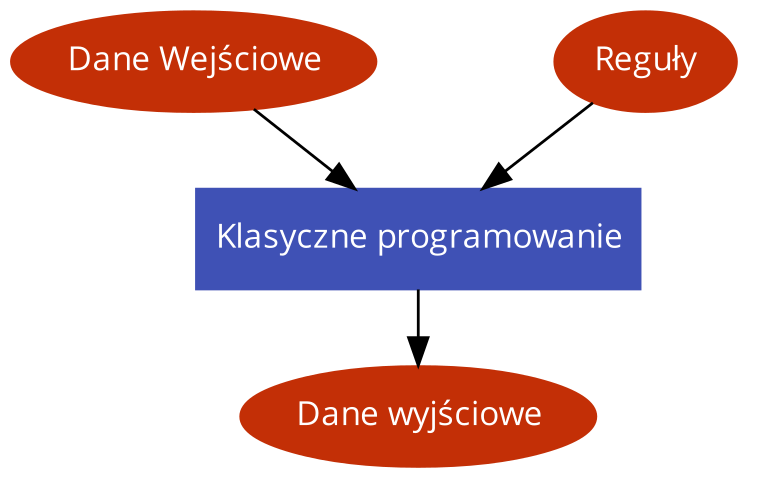
\includegraphics[scale=0.55]{img/Classic.png}
        \caption{Klasyczne programowanie}
        \label{fig:Klasyczne programowanie}    
    \end{center}
    
    \begin{center}
        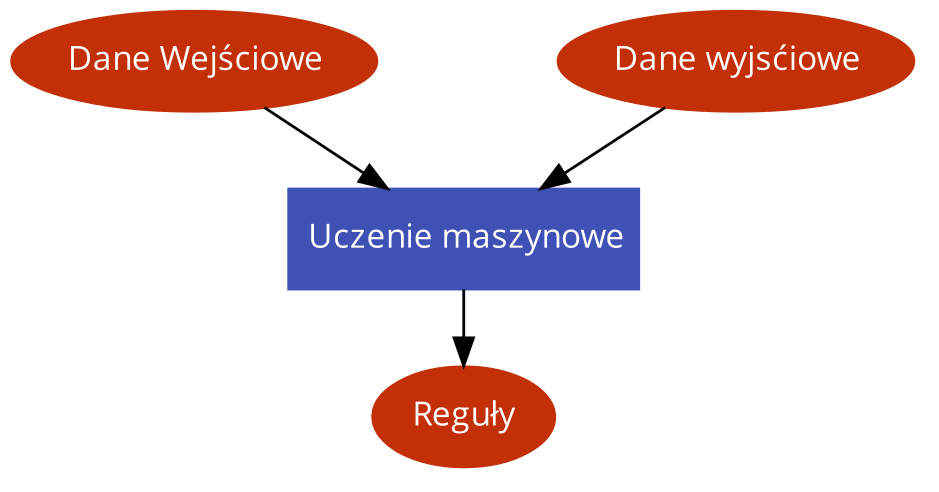
\includegraphics[scale=0.52]{img/ML.png}
        \caption{Uczenie maszynowe}
        \label{fig:Uczenie maszynowe}
    \end{center}
    
\end{figure}

\subsubsection{Klasyfikacja}

Rozróżnienie poszczególnych rodzajów uczenia maszynowego pod względem sposobów działania jest ważne, ponieważ ich zastosowania mogą się znacząco różnić. Systematykę metod uczenia maszynowego można prowadzić pod wieloma względami. Najczęściej wyróżniane są trzy aspekty dzielące techniki uczenia.

Po pierwsze, rozróżniamy metody uczenia ze względu na to czy występuje w nich potrzeba nadzoru ludzkiego. \textbf{Nadzór} w tym wypadku sprowadza się do tego, czy dane uczące posiadają etykiety. \textbf{Etykiety}, czyli oczekiwany wynik (wyjście) odpowiadający konkretnej, uczącej danej wejściowej. Wyróżniamy systemy:

\begin{description}
\item \textbf{Nadzorowane} - dane uczące sporządzone na potrzeby stworzenia algorytmu, oprócz danych wejściowych zawierają rozwiązania. Inaczej mówiąc, zawierają oczekiwane dane wyjściowe.\\Powszechnym zadaniem algorytmów nadzorowanych jest klasyfikacja obiektów oraz regresja. \textbf{Klasyfikacja} polega na przypisaniu obiektu do danej klasy. \textbf{Regresja} to inaczej przewidywanie liczbowego celu.\\ Popularne algorytmy wykorzystujące nadzorowane uczenie maszynowe to:
    \begin{itemize}
        \item Najbliższych sąsiadów (K-nn)
        \item Regresja liniowa
        \item Maszyna wektorów nośnych (SVM)
        \item Drzewa decyzyjne
        \item Las losowy
        \item Sieci neuronowe
    \end{itemize}
    
    \begin{figure}[h!]
    \begin{center}
        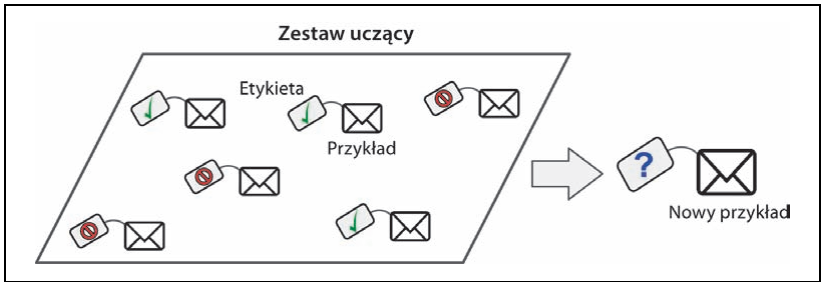
\includegraphics[scale=0.75]{img/oreily.png}
        \caption{Uczenie nadzorowane \cite{oreilly}}
        \label{fig:nadzorowane}    
    \end{center}
    
\end{figure}
\item \textbf{Nienadzorowane} - dane uczące nie posiadają etykiet. Działające na tej podstawie algorytmy są często stosowane do wizualizacji rozkładu danych. Oprócz tego ich typowym zastosowaniem jest wykrywanie anomalii w zbiorach danych. Najpopularniejsze algorytmy związane z nienadzorowanym uczeniem maszynowym to:
    \begin{itemize}
        \item Algorytm centroid-ów (K-Means)
        \item segmentacja danych punktowych oraz rastrowych (DBSCAN)
        \item Grupowanie hierarchiczne (HCA)
    \end{itemize}
    
    \begin{figure}[h!]
    
    \begin{center}
        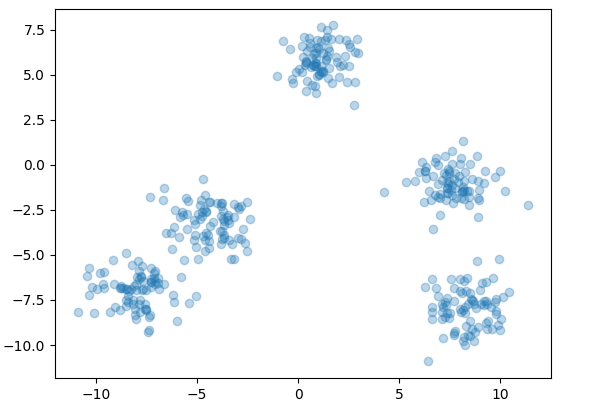
\includegraphics[scale=0.76]{img/unsupervised.png}
        \caption{Zbiór danych bez etykiet}
        \label{fig:nienadzorowane}    
    \end{center}
    
    \begin{center}
        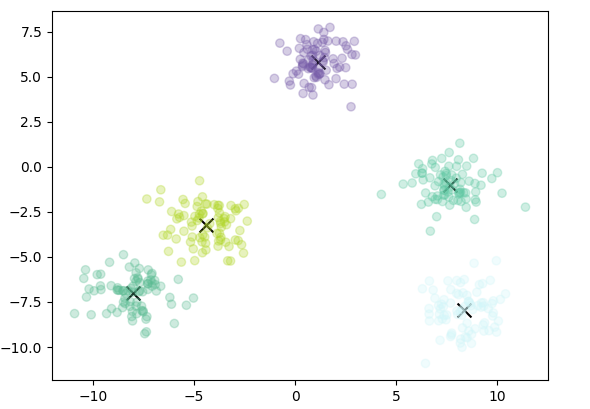
\includegraphics[scale=0.76]{img/kmeans.png}
        \caption{Wizualizacja wyniku algorytmu centroid-ów}
        \label{fig:kmeans}
    \end{center}
    
\end{figure}

\pagebreak
    
\item \textbf{Pół-nadzorowane} - tylko część danych posiada etykiety. Działanie takiego algorytmu można zobrazować na podstawie działania serwisu zdjęć Google. Wyszukują i grupują one z wszystkich zapisanych zdjęć twarze i grupują je osobami, nie wiedząc kto to jest. Następnie użytkownik sam nadaje etykiety do grup zdjęć na przykład w postaci imion, implementując w ten sposób aspekt pół-nadzoru \cite{oreilly}.  

\item \textbf{Uczenie ze wzmocnieniem} - algorytm sam na podstawie dostępnych danych podejmuje wobec nich działania. Jest on regulowany poprzez system nagród i kar. Gdy akcja, którą wykonał była pożądana - jest on nagradzany. W przeciwnym wypadku jest karany. Ten rodzaj uczenia jest powszechnie stosowany w systemach uczących wykorzystywanych w robotyce. W ten sposób robot stopniowo uczy się wykonywać pożądane przez twórców czynności.
\end{description}

Po drugie, możemy rozróżnić rodzaje uczenia maszynowego ze względu na możliwość ciągłego przyswajania nowych danych.
\begin{description}
\item \textbf{Uczenie przyrostowe} - system jest w stanie przyswajać nowe dane uczące w ciągły sposób w trakcie działania. Jest to najlepsze rozwiązanie dla algorytmów potrzebujących adaptować się do nowych danych, które jeszcze nie powstały. Nieprzerwane przystosowywanie się takiego systemu do nowych danych ciągnie za sobą poważny problem. Może on zatracić pożądaną funkcjonalność z czasem, przez wpływ niskiej jakości danych. Jest to zjawisko zwane \textbf{dryfem}. Twórca algorytmu może mu częściowo zapobiec dobierając odpowiedni \textbf{Współczynnik uczenia}. Dzięki niskiemu współczynnikowi uczenia, wpływ dryfu spowodowany potencjalnie zdegenerowanymi, nowymi danymi jest zmniejszony kosztem wolniejszego przystosowywania się do nowych, potencjalnie pożądanych danych.

    \begin{figure}[h!]
    \begin{center}
        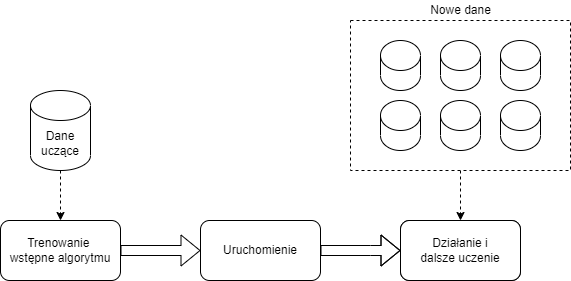
\includegraphics[scale=0.7]{img/przyrostowe.png}
        \caption{Uczenie przyrostowe}
        \label{fig:uczenie_przyrostowe}    
    \end{center}
    \end{figure}

\item \textbf{Uczenie wsadowe} - w procesie uczenia modelu używane są \textbf{wszystkie} dane ze zbioru. 
Każda inicjatywa zmiany działania modelu wymaga jego ponownego, całkowitego wyuczenia. Systemy utylizujące tego typu uczenie, muszą być wyposażone w nietuzinkowe ilości pamięci operacyjnej oraz ogromną moc obliczeniową. Potrzebują one bowiem dużo czasu i zasobów w celu trenowania, zwłaszcza w porównaniu z uczeniem na bieżąco. Algorytmy bazujące na uczeniu przyrostowym mogą ładować kolejne paczki danych uczących, usuwając je, zaraz po użyciu ich w celu uczenia. Ta procedura znacznie zmniejsza zapotrzebowanie sprzętowe.
\end{description}

Na koniec, możemy rozróżnić uczenie maszynowe ze względu na sposób wnioskowania odpowiedzi z danych uczących. Są to:

\begin{description}
\item \textbf{Uczenie z przykładu} - porównujemy nowe instancje danych z wyuczonymi już punktami danych, w ten sposób wnioskując do jakiej grupy danych należy napotkana nowa dana. Aby nie ograniczać algorytmu do odnajdywania odpowiedzi tylko do \underline{identycznych} wejść, jakie posiadał zbiór uczący stosowana jest \textbf{miara podobieństwa}. Pozwala ona na pożądane \textbf{uogólnienie} procesu wnioskowania, biorąc pod uwagę znacznie szerszą gamę danych - te znane oraz grupa danych do nich zbliżonych.

\item \textbf{Uczenie z modelu} - przyjmujemy założenia względem problemu oraz danych wejściowych, wybierając i trenując odpowiednio dobrany \underline{model} (np. regresja liniowa, drzewo decyzyjne, sieć neuronowa i wiele innych). Ucząc model, nadajemy mu zdolność prognozowania na podstawie zależności zachodzących w danych uczących. Powszechnie przyjęte miary pozwalające opisać poprawność działania modelu to \textbf{funkcja dopasowania} oraz \textbf{funkcja kosztu}. Funkcja dopasowania ma za zadanie opisać użyteczność modelu. Uwidocznić to, jak dobrze model współgra z danymi, na podstawie których ma generalizować oraz przewidywać. Funkcja kosztu ma przeciwne zastosowanie. Mierzy ona różnicę pomiędzy oczekiwanymi wynikami, a tymi osiągniętymi przez model.
\end{description}

Wszystkie trzy podziały są od siebie niezależnie i ich mieszanie pomaga osiągnąć różne rezultaty. Dobranie odpowiedniego typu algorytmu jest często kluczowe w celu optymalizacji skuteczności i wydajności jego działania. Dla każdego problemu ze sfery uczenia maszynowego istnieje kilka podejść, które bardziej pasują do natury zagadnienia i będą działać lepiej niż pozostałe. Jeśli potrafimy wysnuć wnioski i skutecznie rozpracować problem, który chcemy rozwiązać uczeniem maszynowym, możemy przyjąć pewne założenia. Pomagają one z doborem strategii działania oraz implementacji systemu bez potrzeby empirycznego szukania najlepszej konfiguracji.

\pagebreak

\subsection{Sieć neuronowa}

\subsubsection{Historia}
\begin{description}
 \item "Początki sztucznej inteligencji sięgają lat czterdziestych ubiegłego stulecia kiedy to opracowano model neuronu w mózgu ludzkim i zwierzęcym (McCulloch i Pitts, 1943) oraz wyjaśniono mechanizm zapamiętywania informacji przez sieć biologiczną. Dalszy rozwój tej nauki zaowocował zaprojektowaniem i zbudowaniem przez Rosenblatta (1958) sztucznej sieci neuronowej zwanej perceptronem. Był to elementarny system wizualny, który mógł być nauczony rozpoznawania ograniczonej klasy wzorów. W tych latach próbowano też pierwszych zastosowań komputerów między innymi do przewidywania pogody, identyfikacji formuł matematycznych, czy analizy elektrokardiogramu.
 
 \item Po publikacji w 1969 książki Minsky'ego i Paperta, w której udowodnili, że jednowarstwowe sieci mają skończone zastosowania, nastąpił odwrót od sieci neuronowych w kierunku systemów ekspertowych. Powrót zainteresowania w połowie lat osiemdziesiątych zapoczątkowały prace ukazujące, że wielowarstwowe, nieliniowe sieci neuronowe nie mają ograniczeń. W tym też okresie rozpoczął się rozwój neurokomputerów, na który także miał wpływ postęp technologii wytwarzania układów scalonych VLSI. Ważnym osiągnięciem są także różnego rodzaju metody uczenia sieci wielowarstwowych np. algorytm wstecznej propagacji błędów." \cite{wstepAGH}.
\end{description}

\subsubsection{Definicja}
\begin{description}
\item "\textbf{Sieci neuronowe}, znane również jako sztuczne sieci neuronowe (ANN) lub symulowane sieci neuronowe (SNN) są częścią funkcji uczenia maszynowego i stanowią podstawę algorytmów uczenia głębokiego. Ich nazwa i struktura są wzorowane na ludzkim mózgu i naśladują sposób, w jaki biologiczne neurony komunikują się między sobą.

Sztuczne sieci neuronowe (ANN) składają się z warstw węzłów, obejmujących warstwę wejściową, jedną lub więcej warstw ukrytych oraz warstwę wyjściową. Każdy węzeł (sztuczny neuron) łączy się z innym i ma powiązaną wagę oraz próg. Jeśli wyjście dowolnego pojedynczego węzła przekracza określoną wartość progową, węzeł ten jest aktywowany podczas wysyłania danych do kolejnej warstwy sieci. W przeciwnym razie żadne dane nie są przekazywane do następnej warstwy sieci." \cite{ibm}.
\end{description}

\pagebreak

\begin{figure}[h!]
    \begin{center}
        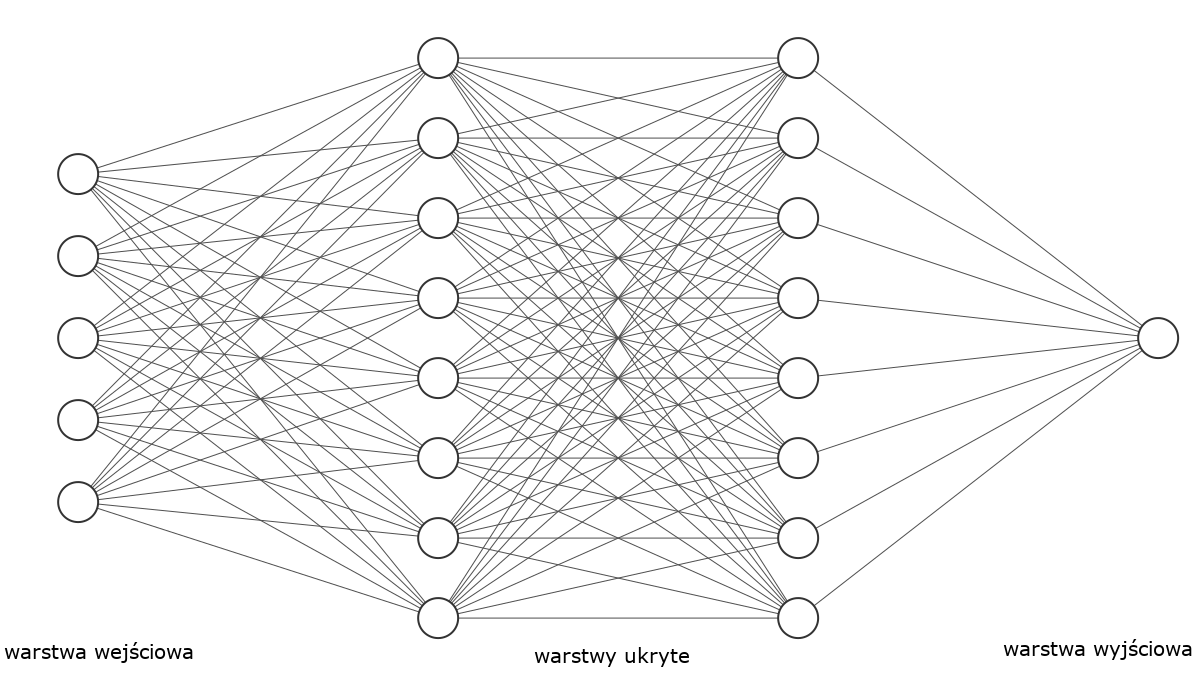
\includegraphics[scale=0.52]{img/nn.png}        
    \end{center}
    \caption{Sieć neuronowa MLP (Perceptron wielowarstwowy)\protect\footnotemark}
    \label{fig:sieć neuronowa}
\end{figure}

\footnotetext{Obraz wygenerowany dzięki narzędziu dostępnemu pod adresem: \url{https://alexlenail.me/NN-SVG}}

\subsubsection{Warstwy sieci neuronowej}
\begin{itemize}
    \label{itm:warstwy}
    \item \textbf{Warstwa wejściowa} - jest nią zawsze pierwsza warstwa. 
    "\null{}Zbiera dane i przekazuje je dalej. [...] Analogicznie jak w przypadku obrazów rejestrowanych np. przez nerwy wzrokowe u człowieka – trafiają do niej nieprzetworzone dane wejściowe" \cite{sztucznainteligencja}
    \item \textbf{Warstwy ukryte} - kluczowe w procesie uczenia. To w nich, szukane są powiązania między poszczególnymi aspektami danej, wprowadzonej z warstwy wejściowej poprzez miary wag, odchyleń i wartości progowych
    \item \textbf{Warstwa wyjściowa} - efekt działania naszego modelu. Ilość węzłów tej warstwy zależy od formatu danych wyjściowych, czyli oczekiwanych przez nas wyników działania sieci (na przykład: lista kolorów wraz z prawdopodobieństwami). Dzięki mierzę prawdopodobieństwa wybierany jest przewidziany wynik wyjściowy modelu - standardowo jest to węzeł z najwyższym rezultatem).
\end{itemize}

\pagebreak

\subsubsection{Perceptron}
Działanie sieci neuronowej najlepiej tłumaczyć zaczynając od opisu jego prostszej formy - \textbf{perceptronu}. To twór złożony z jednego lub wielu \underline{neuronów McCullocha-Pittsa}. Najbardziej trywialny wariant - jedno-neuronowy - potrafi dokonać jedynie klasyfikacji binarnej - określić czy parametry wejściowe należą do danej klasy, czy też nie. Aby otrzymać funkcjonalność klasyfikacji wielu klas należy użyć większej ilości neuronów w warstwie wyjściowej.

\begin{figure}[h!]
    \begin{center}
        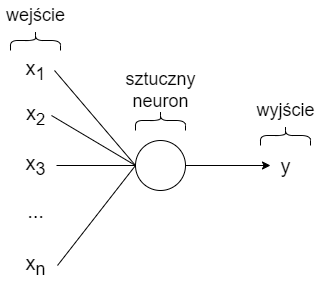
\includegraphics[scale=0.7]{img/perceptron.png}        
    \end{center}
    \caption{Najprostsza forma perceptronu}
    \label{fig:perceptron}
\end{figure}

Bardziej szczegółowy model perceptronu możemy przedstawić zdejmując poziom abstrakcji z neuronu McCullocha-Pittsa. Wtedy model składa się z wejść, ich wag, bloku sumującego, blok aktywacyjnego oraz wyjścia.

\begin{figure}[h!]
    \begin{center}
        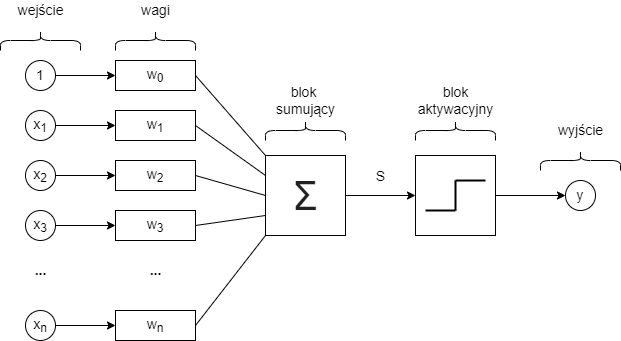
\includegraphics[scale=0.65]{img/perceptron+.png}        
    \end{center}
    \caption{Blokowy schemat perceptronu \cite{wstepAGH}}
    \label{fig:blok_perceptron}
\end{figure}

Działanie tak modelowanego perceptronu charakteryzuję się wzorem:\\

\begin{math}
    \resizebox{0.9\hsize}{!}{$%
    S = \sum_{i = 1}^{m} w_{i}x_{i} + b = w_{1}x_{1} + w_{2}x_{2} + ... + w_{m}x_{m} + b
    $%
    }%
\end{math}\\\\
gdzie:\\
$S$ - wyjście bloku sumującego\\
\begin{math}
x_{i}    
\end{math}
- wartości propagowane z wejścia\\
\begin{math}
w_{i}
\end{math}
- wagi\\
$b$ - odchylenie

Następnie otrzymana suma wchodzi na wejście bloku aktywacyjnego. W bloku zaszyta jest \textbf{funkcja aktywacji}. Może ona przyjmować różną postać i jej wybór należy do projektanta algorytmu. Na wyjściu bloku aktywacyjnego zwracana jest wartość \textbf{1} (neuron jest aktywowany), jeśli wynik sumy przechodząc przez funkcję aktywacji przekroczy wartość progową. W przeciwnym razie zwracane jest \textbf{0} (neuron nie jest aktywowany). Popularnie używane funkcje aktywacji to:

\begin{itemize}
    \item funkcja liniowa
    \item skok jednostkowy
    \item funkcja sigmoidalna
    \item Rectified Linear Unit (ReLU)
\end{itemize}

\begin{figure}[h!]
    \begin{center}
            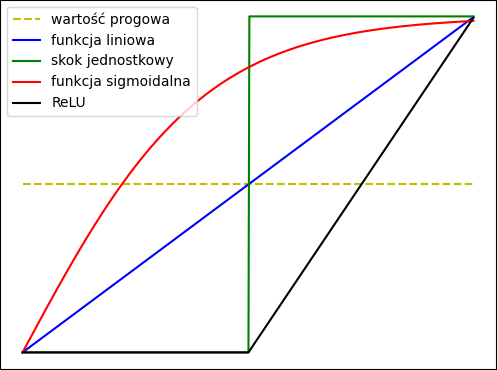
\includegraphics[scale=0.92]{img/aktywacje1.png}        
    \end{center}
    \caption{Funkcje aktywacyjne}
    \label{fig:aktywacje}
\end{figure}


\subsubsection{Perceptron wielowarstwowy (MLP)}

Liczba klas, wobec których perceptron może generalizować jest ograniczona liczbą neuronów w jego warstwie wyjściowej. Oprócz samej liczby neuronów, możemy również zwiększyć ilość warstw perceptronu. Tym sposobem otrzymujemy architekturę \textbf{perceptronu wielowarstwowego}. Jest to, na ten moment, najpopularniejsza architektura sieci neuronowej. Jej schemat przedstawia rysunek \ref{fig:sieć neuronowa}. Składa się ona z jednej warstwy wejściowej, warstw ukrytych złożonych z neuronów McCullocha-Pittsa oraz warstwy wyjściowej. (\ref{itm:warstwy})

Proces uczenia nadzorowanego modelu perceptronu wielowarstwowego jest możliwy dzięki zastosowaniu \textbf{propagacji wstecznej}. To mechanizm polegający na manipulacji wag w celu minimalizacji \textbf{funkcji kosztu}. Często przyjmowaną funkcja kosztu jest błąd średnio-kwadratowy (MSE).

\begin{description}

    \item"\null{}Algorytm \textbf{wstecznej propagacji błędów} polega na takiej zmianie wag sygnałów wejściowych każdego neuronu w każdej warstwie, by wartość błędu dla kolejnych par uczących zawartych w zbiorze uczącym była jak najmniejsza. W tym celu wykorzystywana jest metoda gradientowa najszybszego spadku.
    Schemat krokowy można przedstawić następująco:
    \begin{enumerate}
        \item Inicjalizacja sieci i algorytmu
        \item Obliczanie wartości wyjściowej sieci na podstawie danych
        \item Obliczanie błędu sieci
        \item Korekcja wag
        \item Czy sieć nauczona?
        \item TAK – przejdź dalej
        \item NIE – wróć do punktu 2
        \item Koniec
    \end{enumerate}

    \item Przebieg algorytmu dla wszystkich elementów ciągu uczącego nazywa się \textbf{epoką}." \cite{webarchive}
\end{description}

Funkcja kosztu dana jest ona wzorem:
\begin{center}
\begin{math}
\resizebox{0.42\hsize}{!}{$%
    MSE = \frac{1}{2m}\sum_{i = 1}^{m} ({y}' - y)^{2}
    $%
    }%
\end{math}
\end{center}
gdzie\\
$m$ - ilość próbek\\
$i$ - indeks próbki\\
\begin{math}
{y}'
\end{math}
- wynik otrzymany\\
$y$ - wynik oczekiwany\\

\subsubsection{CNN}

\begin{description}
    \item{
        \textbf{Splotowa sieć neuronowa} (z ang. Convolutional Neural Network - CNN) - to algorytm uczenia maszynowego zaprojektowany na podstawie działania \textbf{kory wzrokowej}. 
        
        Podobnie jak infrastruktura kory wzrokowej, splotowa sieć neuronowa bada obraz etapami. W pierwszym etapie, przetwarzanie obrazu odbywa się na relatywnie małych, \underline{lokalnych polach recepcyjnych}. Części obrazu przetwarzane są wtedy przez neurony reagujące na proste bodźce (linie o różnych orientacjach, krawędzie itp.). Wyjście owych neuronów, jest wejściem dla neuronów, aktywowanych bardziej skomplikowanymi zależnościami w obrazie (kształty, klasy obiektów, kolory itd.), uzyskując stopniowo coraz głębsze i bardziej wyrafinowane powiązania między poszczególnymi aspektami obrazu. Z każdym etapem brane są pod uwagę szersze pola recepcyjne. Mogą się one nakładać na siebie, a łącznie konstruują całe pole wzrokowe \cite{cnn_wroc}.
    }
\end{description}

Wzorowane tym mechanizmem splotowe sieci neuronowe składają się z trzech typów warstw:
\begin{itemize}
    \item Splotowe (z ang. convolution) - "pozwalają na ekstrakcję prostych cech w początkowych warstwach sieci, np. rozpoznają krawędzie o różnej orientacji lub różnokolorowe plamy, a następnie plastry, koła w kolejnych warstwach. Każda warstwa konwolucyjna zawiera cały zbiór filtrów (np. 8 filtrów), a każdy z nich generuje osobną mapę aktywacji 2D. Układamy te mapy aktywacyjne na stercie wzdłuż wymiaru głębokości sieci i produkujemy obraz wyjściowy." \cite{cnn_agh}
    \item Łączące (z ang. pooling) - "\null{}służy do progresywnej redukcji rozmiaru przestrzennego do
zredukowania ilości cech i złożoności obliczeniowej sieci" \cite{cnn_agh}
    \item W pełni połączone lub gęste (FC z ang. fully connected lub dense) - w pełni połączone warstwy, na wzór wielowarstwowego perceptronu.
\end{itemize}

\begin{figure}[h!]
    \begin{center}
        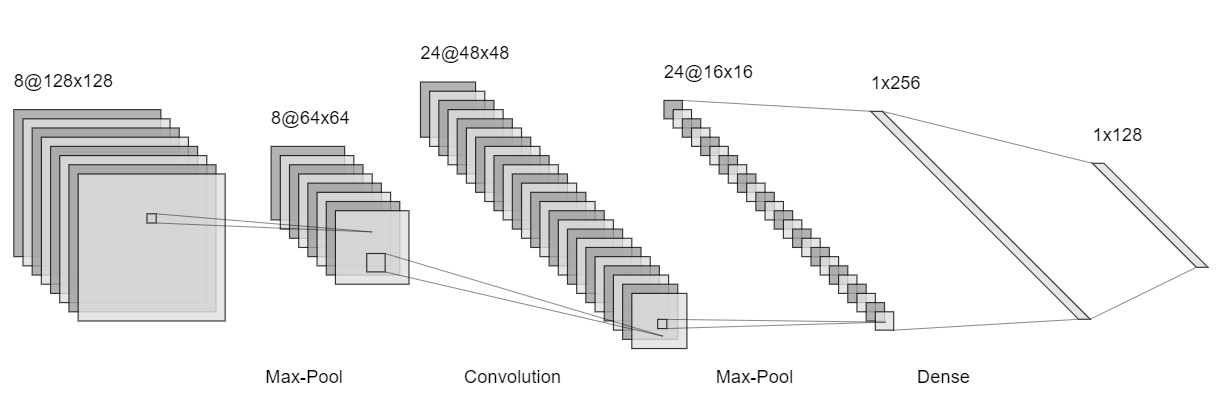
\includegraphics[scale=0.5]{img/cnn_arch_pic.png}
    \end{center}
    \caption{Architektura splotowej sieci neuronowej\protect\footnotemark}
    \label{fig:cnn_arch_pic}
\end{figure}

\footnotetext{Obraz wygenerowany dzięki narzędziu dostępnemu pod adresem: https://alexlenail.me/NN-SVG}

Splotowe sieci neuronowe, tak jak kora wzrokowa, powstały z myślą o danych dwu-wymiarowych (najczęściej obrazy) i właśnie dla tego typu danych są dominującym rozwiązaniem w sferze uczenia maszynowego. W warstwach splotowych wykonywana jest operacja splotu obrazu wejściowego z filtrami, które są przez sieć dostosowywane w celu pozyskania z obrazu poszczególnych cech.

Splotowe sieci neuronowe same w trakcie swojego działania dokonują wyodrębniania cech znaczących. To poważnie zmniejsza liczbę operacji wymaganych w celu optymalizacji ich działania (pozostaję np. selekcjonowanie zbioru danych). Dodatkowo, dzięki swojej architekturze sieci te, wymagają podania mniejszej ilości parametrów w celu konfiguracji. Te dwa fakty znacznie zwiększają przychylność takiego rozwiązania, chociażby ze względu na relatywnie niski wysiłek potrzebny do ich uruchomienia oraz użycia.

Wadą splotowych sieci neuronowych jest to, że przez skomplikowanie i zawarcie w procesie działania wielu złożonych operacji, sieci splotowe są bardzo wolne i wymagające sprzętowo w porównaniu z innymi formami uczenia maszynowego.

Splotowe sieci neuronowe są powszechnie używane w podobnych rozwiązaniach z racji na przystosowanie do danych obrazowych. Na tej technologii oparte są również bardziej skomplikowane i wyrafinowane architekury i modele uczenia maszynowego, na przykład wydajna sieć YOLO (z ang. You Only Look Once) \cite{yolov3}.

\begin{figure}[h!]
    \begin{center}
        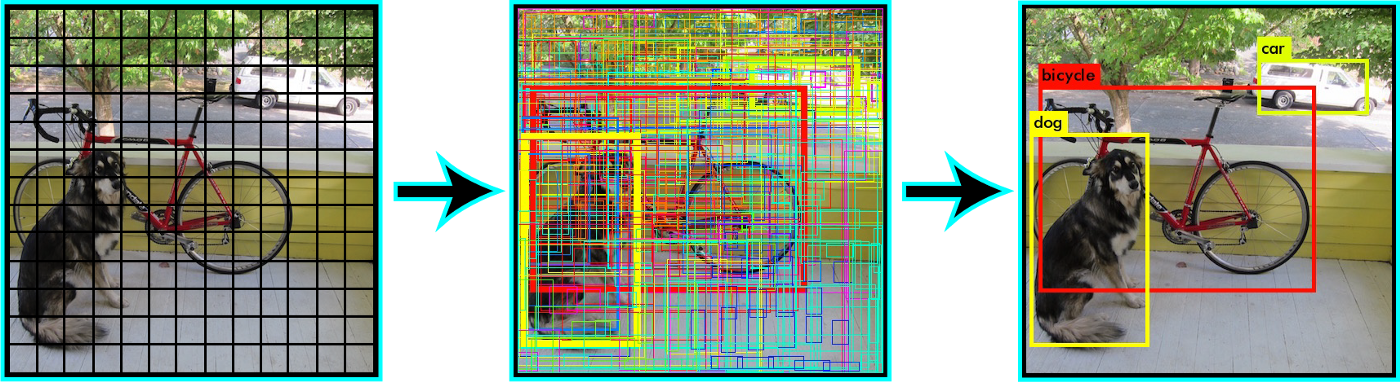
\includegraphics[scale=0.338]{img/yolo_vis.png}
    \end{center}
    \caption{Wizualizacja działania modelu YOLOv3 \cite{yolo_vis}}
    \label{fig:yolo_vis}
\end{figure}
 
 \pagebreak
 
\subsection{Wstępne przetwarzanie danych}
Sieci neuronowe oparte o architekturę perceptronu wielowarstwowego to sieci głębokie, o w pełni połączonych warstwach. Ich wadą jest znaczny wzrost zapotrzebowania na moc obliczeniową oraz pamięć operacyjną wraz z wzrostem liczby parametrów wejściowych. Możemy jednak w dużym stopniu ograniczyć wymogi sprzętowe stosując przetwarzanie danych wejściowych, jeszcze zanim będą one propagowane na wejście sieci. Techniki przetwarzania wstępnego to na przykład: wycinanie, pod-próbkowanie czy wyodrębnianie cech znaczących.

Oprócz tego, realne dane wejściowe, mogą nie być wiernym odwzorowaniem danych uczących. Zdjęcia ruchu ulicznego z reguły mogą zawierać obraz całej drogi i jej okolic, z wieloma pojazdami lub żadnym. Wykrycie pożądanych obiektów jest możliwe dzięki zastosowaniu detekcji obiektów.

\subsubsection{Metody detekcji obiektów}
\begin{description}
\item \textbf{Klasyfikacja} - nadanie etykiety wykrytemu obiektowi, mówiącej do jakiej klasy należy.  

\begin{figure}[h!]
    \begin{center}
        
\includegraphics[scale=0.5]{img/kot.jpg}
    \end{center}
    \caption{Wizualizacja klasyfikacji\protect\footnotemark}
    \label{fig:classification_cat}
\end{figure}

\footnotetext{Użyte zdjęcie kota dostępne pod adresem:      \url{https://rikoland.pl/data/include/img/news/1594756840.jpg}}

\item \textbf{Detekcja} - klasyfikacja obiektu wraz z określeniem jego położenia w obrazie, z reguły wizualizowana za pomocą prostokąta opisanego na obwiedni klasyfikowanego podmiotu.

    \begin{figure}[h!]
    \begin{center}
        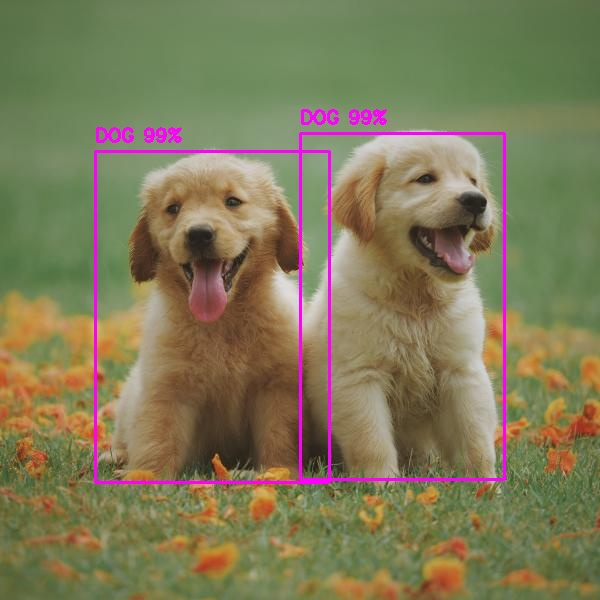
\includegraphics[scale=0.6]{img/detekcja.jpg}
    \end{center}
    \caption{Wizualizacja detekcji\protect\footnotemark}
    \label{fig:detection}
    \end{figure}
    
\footnotetext{Użyte zdjęcie szczeniąt dostępne pod adresem:      \url{https://firsttimedogmom.com/wp-content/uploads/2018/07/Male-vs-Female-Golden-retriever-3.jpg}}

\pagebreak

\item \textbf{Segmentacja} - "proces podziału obrazu na części określane jako obszary (regiony), które są jednorodne (homogeniczne) pod względem pewnych wybranych własności. Obszarami są zbiory pikseli (punktów). Własnościami, które są często wybierane jako kryteria jednorodności obszarów są: poziom szarości, barwa, tekstura." (lub klasy) \cite{wikiseg}.

Segmentacje można podzielić na:
    \begin{itemize}
        
        \item \textbf{Semantyczną} - to rozróżnienie obrazu na segmenty, przy czym obiekty należące od tej samej klasy nie są między sobą rozróżniane. 
        
        \item \textbf{Instancji} - działa jak segmentacja semantyczna, z tą różnicą, że poszczególne instancje tej samej klasy są rozróżniane.
        
    \end{itemize}

    \begin{figure}[h!]
    \begin{center}
        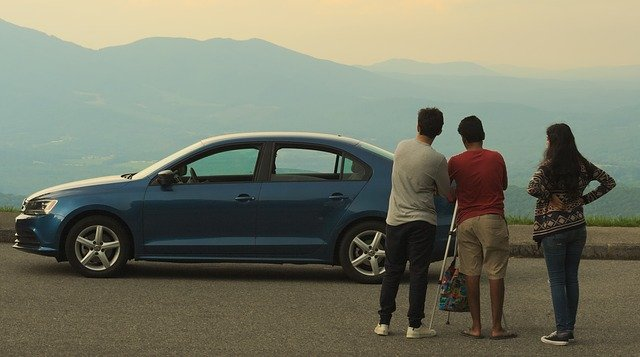
\includegraphics[scale=0.5]{img/car_people.jpg}
    \end{center}
    \caption{Obraz referencyjny\protect\footnotemark}
    \label{fig:ref_seg}
    \end{figure}
    
    \footnotetext{Użyte zdjęcie referencyjne dostępne pod adresem: \url{https://cdn.pixabay.com/photo/2018/04/17/21/56/car-3328898_960_720.jpg}}
    
    \begin{figure}[h!]
    \begin{center}
        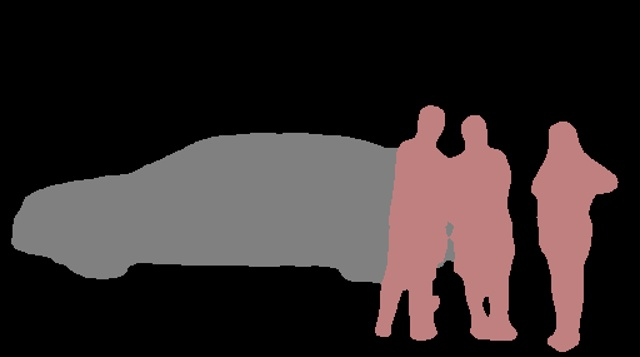
\includegraphics[scale=0.5]{img/car_people_sem.jpg}
    \end{center}
    \caption{Wizualizacja segmentacji semantycznej}
    \label{fig:seg_sem}
    \end{figure}
    
    \begin{figure}[h!]
    \begin{center}
        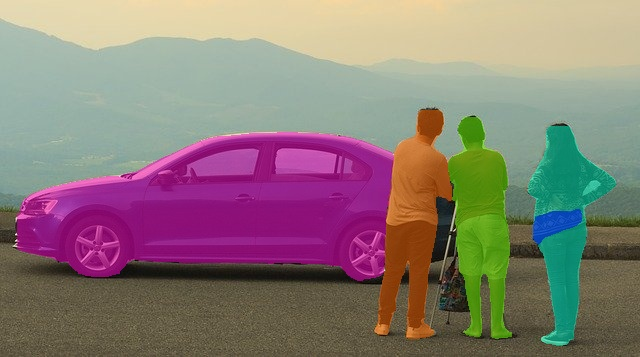
\includegraphics[scale=0.5]{img/car_people_ins.jpg}        
    \end{center}
    \caption{Wizualizacja segmentacji instancji w formie maski nałożonej na obraz referencyjny}
    \label{fig:seg_ins}
    \end{figure}
    
\end{description}

\pagebreak

\subsubsection{Wyodrębnianie cech znaczących}

\textbf{Cechy znaczące} - to wyselekcjonowane części danej wejściowej, na podstawie której model ma wywnioskować potencjalny wynik. Stosujemy konstrukt cech znaczących, aby zniwelować szum mogący powstać przez wpływ niekorzystnych lub nieinteresujących nas elementów wejścia.\\

\begin{figure}[h!]
    \begin{center}
        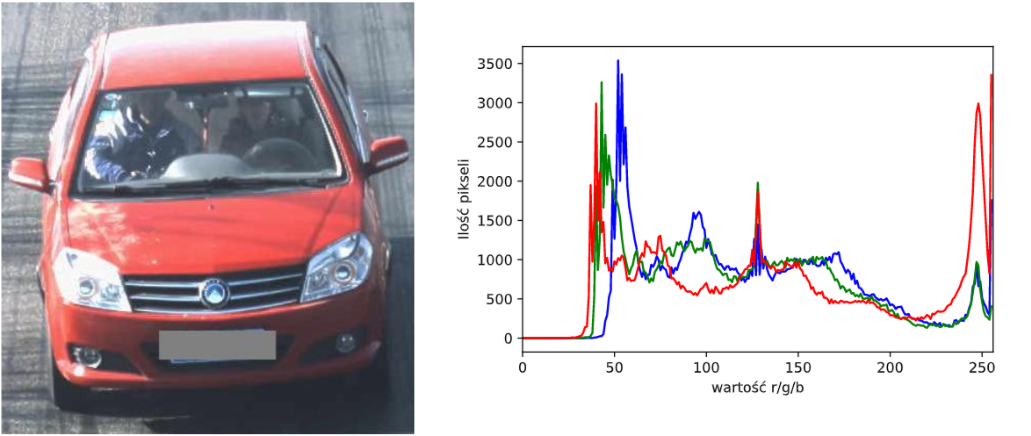
\includegraphics[scale=0.6]{img/feature_extraction.png}        
    \end{center}
    \caption{Ekstrakcja cech znaczących w postaci histogramu kolorów}
    \label{fig:ekstrakcja}
\end{figure}

Wyodrębnianie cech znaczących jest stosowane w celu zmniejszenia wymiarowości napotkanego problemu. W przypadku obrazów wiąże się z ich obróbką, bądź odizolowaniem z nich poszczególnych elementów.

Popularnymi sposobami ekstrakcji cech znaczących są:

\begin{itemize}
    \item Maskowanie elementów obrazu
    \item Wykrywanie obwiedni
    \item Wykrywanie obszarów jednolitych 
    \item Wykrywanie ruchu
    \item Transformacja Hougha i jej pochodne - metoda odszukiwania regularnych kształtów (oryginalnie prostych)
    \item Filtrowanie (w tym górno oraz dolnoprzepustowe)
    \item Dopasowywanie wzorcowe
\end{itemize}


\subsection{Statystyka dotycząca kolorów aut na polskich drogach}

Gama kolorów aut jest bardzo szeroka. Jednak jest ona zdominowana przez kilka najpopularniejszych barw.

Czołowa dziesiątka najpopularniejszych kolorów \cite{autocentrum}:
\begin{enumerate}
    
    \item Srebrny – 25\%
    \item Czarny – 23\%
    \item Biały – 16\%
    \item Szary – 13\%
    \item Niebieski – 9\%
    \item Czerwony – 8\%
    \item Brązowy i beżowy – 4\%
    \item Zielony – 1\%
    \item Żółty i złoty – 1\%
    \item Inne – poniżej 1\% 
\end{enumerate}

Wyciągając dalsze wnioski z owej statystyki, można zauważyć, że biorąc pod uwagę jedynie osiem kolorów: srebrny, czarny, biały, szary, niebieski, czerwony, cyjanowy, zielony i żółty - otrzymamy ponad \textbf{93\%} pokrycia barw wszystkich aut. Właśnie te kolory są dostępne w użytym zbiorze danych.

Kolory srebrny i szary są uwzględnione jako jeden kolor z uwagi na trudność ich rozróżnienia. Zdjęcia w zbiorze danych borykają się z wieloma problemami wpływającymi znacznie na ich jakość (opisane dogłębnie w podrozdziale \ref{sec:dataset}). Metaliczny połysk srebra jest niemal zawsze w warunkach drogowych zatracany przez brud, kurz, warunki atmosferyczne, oświetlenie i jakość zdjęć. To sprawia, że w większości przypadków, te dwa kolory są nierozróżnialne z punktu widzenia ludzkiego oka, a tym bardziej programowo.

\subsection{Użyty zbiór danych}
\label{sec:dataset}

Dane użyte do trenowania modelu uczenia maszynowego pochodzą z publikacji naukowej dotyczącej tematyki rozpoznawania koloru aut \cite{chen_ref}.\\

Zbiór danych składa się z 15601 obrazów przedstawiających pojazdy na drogach miejskich widziane od przodu. Zdjęcia zostały wykonane przy pomocy kamery o rozdzielczości 1920x1080.

\begin{figure}[h!]
    \begin{center}
        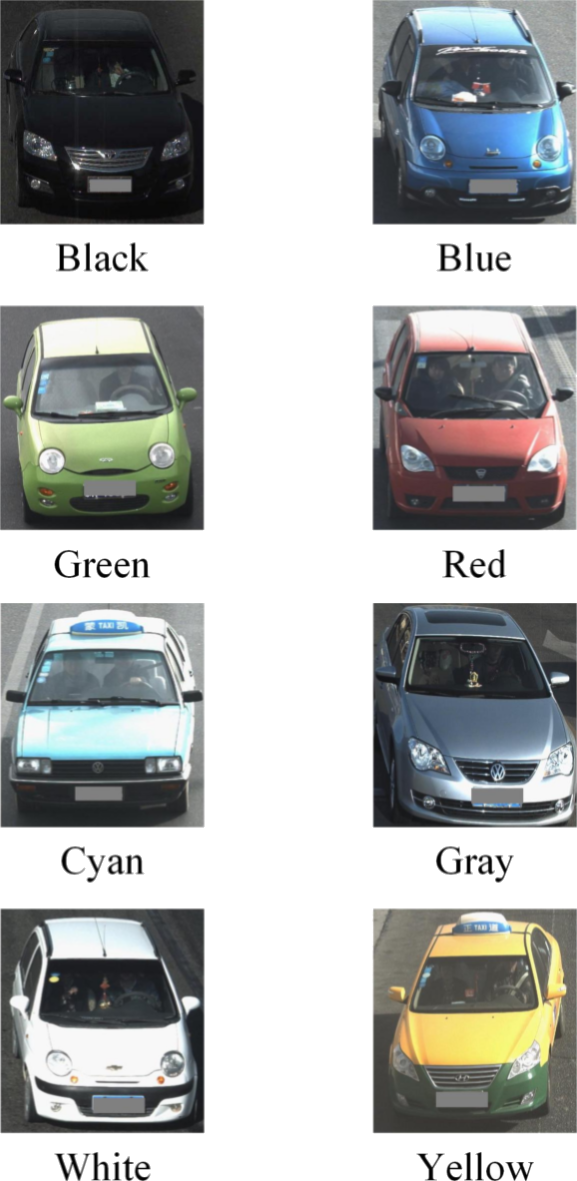
\includegraphics[scale=0.73]{img/dataset.png}        
    \end{center}
    \caption{Przykładowe obrazy ze zbioru danych wraz z ich etykietami}
    \label{fig:przykładowe obrazy}
\end{figure}

\pagebreak

Zbiór jest obarczony wieloma problemami wpływającymi na wynikowe działanie trenowanego nim modelu:

\begin{itemize}
    \item Składa się jedynie ze zdjęć pojazdów z widoku frontalnego, co sprawia, że model optymalnie wywnioskuje jedynie samochody widziane z podobnej perspektywy. Przez to jest ograniczony.
    \item Część zdjęć jest widocznie zniekształcona przez zastałe warunki atmosferyczne, oświetlenie oraz wszelakiego rodzaju rozmycie obrazu. Przez to, rozróżnienie par kolorów zbliżonych do siebie (na przykład szary-czarny i szary-biały) jest problematyczne.
    \item Obrazy zawierają w sobie element tła, którego negatywny wpływ na ekstrahowany histogram kolorów jest zauważalny w wynikowym działaniu algorytmu. Programowe usunięcie tła to bardzo kosztowna operacja pod względem zasobów. Jest to szczególnie dotkliwe dla wydajności przy działaniu programu na plikach wideo.
    \item Niektóre zdjęcia, przez prawdopodobny wpływ czynnika ludzkiego w procesie manualnej klasyfikacji, mają niepoprawnie przypisane kolory.
    \item W zbiorze istnieją zdjęcia pojazdów, których elementy karoserii są różnych kolorów. Fakt ten sprawia, iż wyuczony model może zostać zdegenerowany przez zawarcie w histogramach kolorów innej barwy, niż koloru przypisanego do danego zdjęcia.
\end{itemize}

% \subsection{Informacja o kolorze pozyskiwana z obrazu}

% Informacje o obrazie w postaci numerycznej można pozyskać dzięki użyciu biblioteki OpenCV w języku Python.
% Metoda \textbf{cv2.imread()} zwraca informacje o wartościach kanałów \textbf{RGB} każdego piksela w postaci zagnieżdżonej listy. Wykaz wspieranych formatów obrazów metody jest liczny, a co ważniejsze zawiera w sobie formaty \textbf{.jpg} oraz \textbf{.png}. Jest również możliwe użycie OpenCV do przetworzenia na dane numeryczne plików wideo, między innymi \textbf{.mp4} i \textbf{.avi}.

% \begin{lstlisting}[language=Python, caption=Przykład wczytania obrazu]
% import cv2  # Korzystamy z biblioteki openCV

% file_path = r'../assets/0197.jpg'
% image = cv2.imread(file_path)

% print(image.shape)
% print(image)
% \end{lstlisting}


% \begin{lstlisting}[language=Python, caption=Wynik wczytania obrazu]
% (426, 408, 3)  # wymiary obrazu (426, 408) oraz kanaly RGB (3)
% [[[193 185 178]  # Tablica wartosci kanalow RGB poszczegolnych pikseli
%   [202 194 187]  
%   [204 196 189]
%   ...
%   [131 127 116]
%   [132 128 117]
%   [132 128 117]]]
% \end{lstlisting}

% \begin{lstlisting}[language=Python, caption=Wizualizacja wczytanego obrazu]
% import cv2

% file_path = r'../assets/0197.jpg'
% image = cv2.imread(file_path)  # Wczytanie obrazu

% cv2.imshow('Window title', image)  # Wyswietlenie obrazu w oknie o tytule 'Window title'
% cv2.waitKey(0)  # Instrukcja wstrzymujaca zamkniecie okna z obrazem az uzytkownik kliknie dowolny przycisk
% \end{lstlisting}

% \begin{figure}[h!]
%     \begin{center}
%         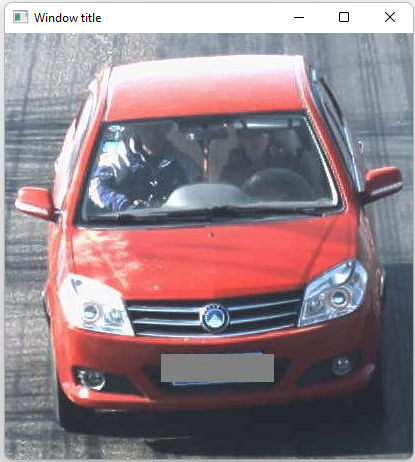
\includegraphics[scale=1.1]{img/0197-windowed.png}        
%     \end{center}
%     \caption{Wczytany obraz pokazany w oknie}
%     \label{fig:wczytanie obrazu}
% \end{figure}

% \pagebreak

% Do wczytywania plików wideo lub obrazu na żywo z wejścia wideo komputera używamy klasy \textbf{cv2.VideoCapture()}. Wczytujemy dzięki niej kolejne klatki pliku wideo. Wynik wczytania każdej z klatek jest tożsamy do wyniku funkcji \textbf{cv2.imread()} na pojedynczym obrazie.\\
% Przykład jej użycia:

% \begin{lstlisting}[language=Python, caption=Wczytanie oraz wizualizacja wideo]
% import cv2

% video_file_path = r'../assets/blue_car.mp4'

% cap = cv2.VideoCapture(video_file_path)

% while cap.isOpened():  # Jesli udalo sie otworzyc plik, powtarzaj operacje czytania + przetwarzania + wizualizuj
%     success, img = cap.read()  # Czytaj kolejna klatke

%     # Przerwij petle jesli napotkany zostanie koniec pliku
%     if not success:
%         break

%     # Potencjalne operacje na obrazie

%     cv2.imshow("Window title", img)  # Wyswietl klatke w oknie o tytule  'Window title'
%     cv2.waitKey(1)  # 1 milisekundowa przerwa pomiedzy klatkami 

% cap.release()  # Zwolnij zasoby
% cap.destroyAllWindows()  # Zamknij okna otwarte przez openCV 
% \end{lstlisting}
\section{Aktualny stan wiedzy}

Algorytmy opierające się o sztuczną inteligencję cieszą się dużą popularnością ze względu na ich ogromną gamę zastosowań. Rozwiązania związane z uczeniem maszynowym zrewolucjonizowały w ostatnich dekadach wiele dziedzin nauki i prac badawczych. Technologie te, pozwoliły w niezliczonej liczbie przypadków przewyższyć konkurencyjne rozwiązania pod względem skuteczności i wydajności. 
Świadectwem tego, jest na przykład inteligentne nad-próbkowanie, wydatnie zwiększające jakość obrazów oraz filmów na podstawie jedynie ich kopii o niskiej rozdzielczości. 

Dodatkowo, sztuczna inteligencja umożliwiła opracowanie wielu funkcjonalności, którym klasyczne podejście do programowania nie jest fizycznie w stanie dorównać (w skończonej liczbie instrukcji). Przykładem tego, jest przewidywanie trendów i specyficzne rodzaje detekcji.

\subsection{Istniejące rozwiązania i prace naukowe}

Na dzień dzisiejszy istnieje wiele różnych implementacji systemów wykrywania koloru pojazdów. Reinterpretacji tego problemu pojawia się z biegiem czasu coraz więcej. Fakt ten wynika z rosnącego zainteresowania oraz zapotrzebowania na rozwój algorytmów opartych o uczenie maszynowe w obszarze przetwarzania obrazów, które jest dominującym narzędziem w tej dziedzinie.

Prace naukowe z dziedziny rozpoznawania koloru pojazdów przedstawiają swoiste podejścia do implementacji algorytmu. Proponują oraz uzasadniają przyjętą konfigurację uczenia maszynowego, oferując coraz lepsze wyniki. Twórczość autorów w kwestii optymalizacji algorytmów owocuję nietuzinkową skutecznością i wydajnością otrzymanych rozwiązań.


% Vehicle Color Recognition on Urban Road by Feature Context
% \subsubsection{Regresja liniowa} -> alternatywny podtytuł
\subsubsection{"\null{}Rozpoznawanie koloru samochodów osobowych w ruchu drogowym przez wyodrębnienie cech znaczących" \cite{chen_ref}}
Rozwiązanie opracowane przez Pan Chen, Xiang Bai, Wenyu Liu. Ta praca naukowa jest szczególnie znacząca, ponieważ użyty w niej zbiór danych trenujących jest publicznie dostępny i wiele innych prac naukowych używa go w celach ewaluacyjnych dla swoich rozwiązań.

Kroki zaimplementowany przez kadrę algorytmu to:
\begin{itemize}
    \item Detekcja pojazdu
    \item Usunięcie rozmycia i zamglenia z obrazu
    \item Uwydatnienie kolorów
    \item Wyodrębnienie z obrazu obszaru zainteresowania (ROI, z ang. Region of interest)
    \item Użycie modelu regresji liniowej (SVM, z ang. support vector machine, trenowanej również na ROI pozyskanych z danych uczących) w celu wyznaczenia dominującego koloru w obszarze zainteresowania
\end{itemize}

\begin{figure}[h!]
    \begin{center}
        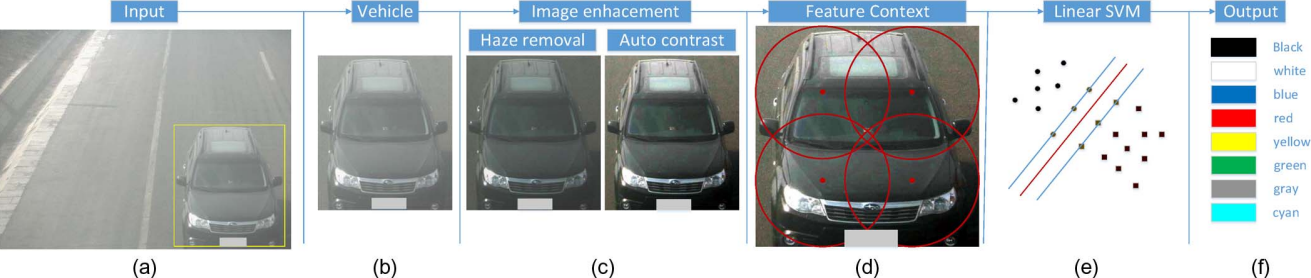
\includegraphics[scale=0.48]{img/chen.png}
    \end{center}
    \caption{Kroki algorytmu: a) obraz wejściowy, b) wynik detekcji i wycięcia, c) kolejno usunięcie zamglenia i uwydatnienie kolorów, d) ROI, e) trenowanie/testowanie modelu SVM, f) wynik działania algorytmu}
    \label{fig:chen_algo}
\end{figure}

Algorytm ten, cieszy się raportowaną przez twórców skutecznością w granicach \textbf{92\%}. Głównym założeniem projektantów, było umożliwienie działania programu zarówno na zdjęciach jak i obrazie wideo. Przetwarzanie wstępne w postaci usuwania niedoskonałości i wyznaczenia ROI jest niezwykle kosztowne pod kątem zasobów sprzętowych. Niska wydajność uniemożliwia satysfakcjonujące działanie algorytmu na obrazie wideo (niska liczba klatek na sekundę). Z tego powodu, został użyty model regresji liniowej. Model ten, jest mniej wymagający sprzętowo w porównaniu do modelu sieci neuronowej. Dzięki temu kompromisowi, autorom udało się uzyskać wysoką skuteczność w połączeniu z zadowalającą wydajnością algorytmu.

% Vehicle Color Recognition using Convolutional Neural Network
% \subsubsection{Splotowa sieć neuronowa}
\subsubsection{"\null{}Rozpoznawanie koloru samochodów osobowych używając splotowej sieci neuronowej" \cite{Su2015/12}}
Podejście zaproponowane przez Reza Fuad Rachmadi oraz Ketut Eddy Purnama.

Algorytm oparty jest na:
\begin{itemize}
    \item Konwersji obrazu do przestrzeni HSV (z ang. Hue Saturation Value) oraz CIELab
    \item Przepuszczenia skonwertowanych obrazów przez splotową sieć neuronową (CNN)
\end{itemize}

\pagebreak

\begin{figure}
    \begin{center}
        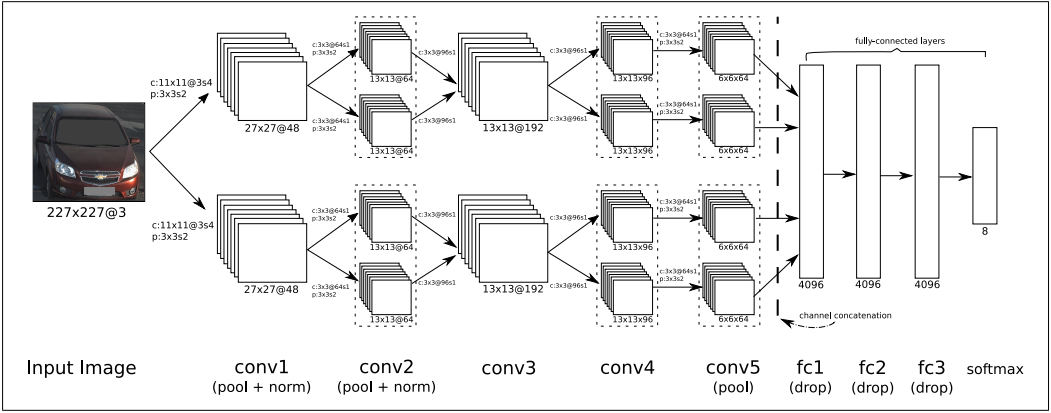
\includegraphics[scale=0.6]{img/cnn_arch.png}
    \end{center}
    \caption{Architektura CNN użytej w pracy naukowej}
    \label{fig:cnn_arch}
\end{figure}

Użyta splotowa sieć neuronowa została wytrenowana według procedury wprowadzonej przez Alexa Krizhevskiego. Polega ona na zmniejszaniu kroku modyfikacji współczynnika uczenia wraz z kolejnymi iteracjami uczenia o stałą wartość (poczynając od pewnej ustalonej iteracji). W przypadku artykułu stała to 10.

Splotowe sieci neuronowe są zazwyczaj używane do klasyfikacji pod kątem kształtu podmiotu. Może ona jednak zostać użyta do klasyfikacji pod względem koloru, dzięki konwersji do przestrzeni uwydatniających rozkład kolorów w obrazie, takich jak HSV oraz CIELab. 

Te zabiegi pozwoliły autorom algorytmu osiągnąć skuteczność 94\%, czyli o 2\% większą od rozwiązania Pan chen, Xiang Bai oraz Wenyu Li, na tym samym zbiorze danych. 

Wadą tego rozwiązania jest czas trenowania modelu CNN, przez co autorzy trenowali i testowali algorytm jedynie na \underline{połowie} obrazów ze zbioru. Nawet mimo tego ograniczenia liczebności danych uczących, trenowanie modelu przebiegało przez okres około 4 dni, używając potężnej karty graficznej w celu zrównoleglenia wymagających operacji.

Z macierzy pomyłek udostępnionej przez twórców rozwiązania, możemy wnioskować z jakimi kolorami algorytm radził sobie najlepiej, a z jakimi miał problemy. Większość kolorów cieszy się wysoką skutecznością rozpoznawania przez model, jednak kolor szary był w około 10\% mylony z kolorem białym, a zielony z szarym oraz czarnym w aż 15\% przypadków testowych.

\begin{figure}[h!]
    \begin{center}
        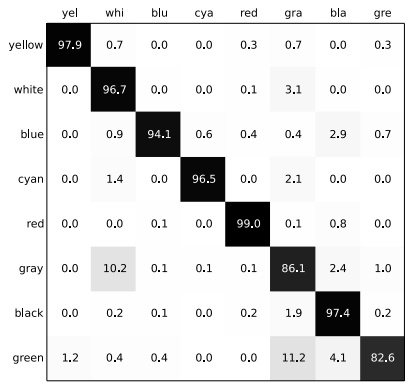
\includegraphics[scale=1.2]{img/confusion_cnn.png}
    \end{center}
    \caption{Macierz pomyłek rozwiązania}    
    \label{fig:confusion_cnn}
\end{figure}

% Vehicle Color Recognition in The Surveillance with Deep Convolutional Neural Networks
% \subsubsection{Głęboka splotowa sieć neuronowa}
% \subsubsection{"\null{}Rozpoznawanie koloru samochodów osobowych w monitoringu ruchu drogowego z użyciem głębokich splotowych sieci neuronowych" \cite{DBLP:journals/corr/RachmadiP15}}

\pagebreak

\subsection{Aplikacje non-profit i open source}
Wiele entuzjastów dziedziny uczenia maszynowego oraz przetwarzania obrazów zdecydowało się na implementację swojej własnej wersji algorytmu wykrywania kolorów pojazdów drogowych. Rozwiązania te, są z reguły dostępne w formie kodu otwartego źródła w publicznych repozytoriach.

Kilka przykładów:
\begin{itemize}
    \item \textbf{Vehicle-Make-Color-Recognition} użytkownika nikalosa. Rozwiązanie napisane w pełni w języku python i bibliotece Pytorch, opiera się na \underline{uczeniu transferowym}. To podejście koncentruje się na zachowaniu wiedzy pozyskanej przez model podczas uczenia i użycie jej w kolejnej operacji uczenia. Użyty model to resnext101 (32x8d). Oprócz koloru, algorytm rozpoznaje również markę pojazdu. \cite{nikalosa}
    
    \item \textbf{car-color-identification} użytkownika sergorl. To implementacja rozpoznawania koloru aut używająca splotowych sieci neuronowych opisanych w \textbf{Keras}, będącej interfejsem do biblioteki Tensorflow. \cite{sergorl}
    
    \pagebreak
    
    \item \textbf{Vehicle-Detection-And-Color-Classification} użytkownika SKsaqlain. Do detekcji samochodów używane jest rozróżnienie statycznych obiektów w kolejnych klatkach obrazu wideo. Po odizolowaniu samochodu z obrazu, używana jest klasyfikacja za pomocą algorytmu centroidów (K-means) na znormalizowanej macierzy kolorów wyodrębnionej z obszaru zajmowanego przez wykryte auto. \cite{saqlain}
\end{itemize}

\subsection{Aplikacje komercyjne}
Istnieje wiele komercyjnych systemów pozwalających na kompleksową identyfikację pojazdów. 
Detekcja koloru samochodu jest używana w tym celu komplementarnie z rozpoznawaniem:
\begin{itemize}
    \item Marki
    \item Modelu
    \item Typu pojazdu (auto osobowe, dostawcze, ciężarowe, dwuślad)
    \item Zawartości tablic rejestracyjnych
\end{itemize}

Kilka przykładowych, komercyjnych systemów pozwalających na kompleksową identyfikację pojazdów to: 
\begin{itemize}
    \item \textbf{Carmen® MMR} firmy \textbf{Adaptive Recognition} (wcześniej znanej jako ARH) \cite{carmen}
    \item \textbf{Asura} firmy \textbf{Milestone Systems A/S} \cite{asura}
    \item \textbf{numberOK SDK LPR} firmy \textbf{FF Group} \cite{numberok}
    \item Rozwiązanie firmy \textbf{Kuartis} (implementuje jedynie rozpoznawanie koloru i tablic rejestracyjnych pojazdów) \cite{kuartis}
\end{itemize}

\section{Implementacja}
W tym rozdziale przedstawiona zostanie implementacja w postaci modułowej. Na początek jednak, warto wyróżnić dostępne biblioteki oraz te użyte w realizacji projektu. Każda operacja wchodząca w skład algorytmu rozpoznawania koloru samochodów osobowych zostanie przybliżona. Oprócz znaczenia i krótkiego opisu każdego z modułów, przekazana zostanie również jego programowa implementacja w postaci krótkiego listingu kodu źródłowego.

\subsection{Dostępne i użyte technologie}

Do wykonania projektu użyty został język programowania \textbf{Python}. Ten wybór uzasadniony jest przez:
\begin{enumerate}
    \item Osobiste obycie oraz doświadczenie z językiem 
    \item Ogromną dostępność bibliotek oraz rozwiązań pozwalających na implementację:
        \begin{itemize}
            \item Przetwarzania obrazu (OpenCV, numpy, scikit-image, pillow)
            \item Uczenia maszynowego (scikit-learn, tensorflow, keras)
            \item Ogólnej wygody i wydajności przy pracy ze zbiorami danymi (numpy, pandas)
            \item Wykrywania obiektów z obrazu (OpenCV, OpenCV + YOLOv3 \cite{yolov3})
        \end{itemize}
    \item Każde z używanych narzędzi cieszy się rozbudowaną, nieustannie utrzymywaną dokumentacją oraz wsparciem.
\end{enumerate}

Kolejne technologie wraz z ich implementacjami przytaczane będą zgodnie z kolejnością ich użycia w algorytmie.

\subsection{Wczytanie zbioru danych}
Wczytujemy do pamięci operacyjnej obrazy ze zbioru danych za pomocą bibliotek \textbf{OpenCV} oraz \textbf{os}.
Wbudowana biblioteka języka python - \textbf{os}, pozwala na operacje na plikach oraz folderach (także listowanie ich zawartości).

\begin{lstlisting}[language=Python, caption=Wczytanie zbioru danych]
import os
import cv2 as cv

data_path = r'assets/train' # Glowny folder danych
data = { "images": [], "label": [] }

for subdir in os.listdir(data_path): # Przejscie przez kazdy podfolder
    current_path = os.path.join(data_path, subdir)

    for file_name in os.listdir(current_path): # Przejscie przez kazdy plik w podfolderze
        image_path = os.path.join(current_path, file_name)
        image = cv.imread(image_path)
        data["imagees"].append(image)
        data["label"].append(subdir)
\end{lstlisting}

W zmiennej \textbf{data} (typu słownik) agregowane są etykiety danych - \textbf{label} - oraz dane liczbowe wczytanych obrazów - \textbf{images} (każdy obraz to tablica wartości kanałów RGB każdego piksela). Program zakłada strukturę plików, w której w folderze \textbf{assets/train} znajdują się podfoldery, których nazwy to etykiety zawartych w nich obrazów.

\subsection{Wykrywanie obiektów}
Do detekcji pojazdów użyta została biblioteka \textbf{OpenCV} w połączeniu z publicznie dostępnym, wytrenowanym modelem \textbf{YOLOv3}. Model ten został wytrenowany na podstawie zbioru danych "\null{}Pospolitych Obiektów w Kontekście" (COCO, z ang. Common objects in context) \cite{coco}. Oprócz samochodów, owy zbiór danych zawiera w sobie 79 innych klas obiektów.

Działanie obu bibliotek jest komplementarne w procesie detekcji. Za pomocą OpenCV tworzymy głęboką sieć neuronową, której nadajemy wagi dostępne w wyuczonym modelu YOLOv3. Przepuszczamy obrazy przez głęboką sieć, odnajdując wszystkie instancje pożądanej klasy. W wyniku otrzymujemy współrzędne każdej odnalezionej instancji w obrazie w formacie wymiarów prostokąta opisanego na instancji (wysokość, szerokość oraz współrzędne lewego, górnego rogu prostokąta względem lewego górnego rogu oryginalnego obrazu).\\

\begin{lstlisting}[language=Python, caption=Przetworzenie obrazu za pomocą głębokiej sieci neuronowej]
import cv2 as cv
# Inicjalizacja glebokiej sieci neuronowej
deep_neural_network = cv.dnn.readNetFromDarknet(
                    r"config/yolov3-320.cfg", 
                    r"config/yolov3.weights")
# Funkcja przetwarzajaca obraz za pomoca sieci            
def dnn_passthrough(image):
    blob = cv.dnn.blobFromImage(
            image, 1 / 255, # dane liczbowe obrazu oraz zadane skalowanie
            (width_height, width_height), # rozmiary powstalego blobu
            [0, 0, 0], 1, crop=False) # konwersja z formatu BGR do RGB
    deep_neural_network.setInput(blob)
    layers_names = deep_neural_network.getLayerNames()
    output_names = [(layers_names[i - 1]) 
                for i in deep_neural_network.getUnconnectedOutLayers()]
    return deep_neural_network.forward(output_names)
\end{lstlisting}

Tworzymy model głębokiej sieci neuronowej za pomocą metody biblioteki OpenCV \textbf{readNetFromDarknet}, której jako parametry podajemy pliki konfiguracyjne modelu YOLOv3. 

Funkcja \textbf{dnn\_passthrough} służy do przetworzenia obrazu przez ową sieć. Najpierw obraz konwertujemy do formatu \textbf{blob}. W tym przypadku oznacza to jedynie skalowanie obrazu o współczynnik 1/255 (zmniejszenie) oraz zamiana kolejności kanałów kolorów z formatu BGR do RGB (funkcję biblioteki OpenCV standardowo operują na danych liczbowych obrazu w układzie BGR). Przejście do formatu blob jest wykonywane, ponieważ sieci neuronowe dostępne w OpenCV były optymalizowane pod kątem właśnie tego formatu. Następnie mówimy metodzie \textbf{forward}, wartości których warstw sieci nas interesują podając ich nazwy jako parametr. Oczywiście interesują nas jedynie warstwy wyjściowe (wynik sieci neuronowej) - podajemy więc zmienną \textbf{output\_names}, zawierającą nazwy warstw wyjściowych.

\begin{lstlisting}[language=Python, caption=Znalezienie wymiarów prostokątów opisanych na wykrytych siecią obiektach]
import cv as cv2, numpy as np

def find_objects(dnn_outputs, image):
    height, width, _ = image.shape # Rozmiary obrazu wejsciowego
    bounding_boxes, class_indexes, confidences = [], [], []

    for output in dnn_outputs:
        for determinant in output:
            scores = determinant[5:]
            class_index = np.argmax(scores)
            confidence = scores[class_index]

            if confidence > confidence_threshold and class_names[class_index] == 'car':
                w = int(determinant[2] * width)
                h = int(determinant[3] * height)
                x = int((determinant[0] * width) - w / 2)
                y = int((determinant[1] * height) - h / 2)
                bounding_boxes.append([x, y, w, h])
                class_indexes.append(class_index)
                confidences.append(float(confidence))

    indices = cv.dnn.NMSBoxes(
        bounding_boxes,
        confidences,
        confidence_threshold,
        non_maximum_suppresion_threshold)

    return [bounding_boxes[i] for i in indices]
\end{lstlisting}

\pagebreak

Funkcja \textbf{find\_objects} przechodzi przez listę wszystkich wyników detekcji głębokiej sieci. Jeśli wykryty został samochód oraz pewność detekcji jest wyższa niż zadany przez nas próg, wyliczane zostają współrzędne lewego górnego rogu prostokąta opisanego na wykrytym obiekcie względem lewego górnego rogu oryginalnego obrazu oraz szerokość i wysokość tego prostokąta. Współrzędne prostokąta, wraz z pewnościami ich detekcji oraz klasą, która została wykryta (dla nas to zawsze samochód) są przetrzymane w zmiennych. 

Na podstawie współrzędnych prostokąta, pewności i klasy detekcji oraz dodatkowo zadanego progu spłaszczania prostokątów, metoda \textbf{NMSBoxes} redukuje nachodzące na siebie, redundantne prostokąty. Dzięki tej operacji, wynik wyjściowy działania funkcji find\_objects to pojedynczy prostokąt dla każdego wykrytego obiektu.

\begin{lstlisting}[language=Python, caption=Użycie zaimplementowanej detekcji i jej wizualizacja]
import cv2 as cv

image_path = r'assets/0197.jpg'
image = cv.imread(image_path)
outputs = dnn_passthrough(image)

try:
    boxes = findObjects(outputs, image)
except:
    print("Couldn't find a car in given frame")
    
for box in boxes:
    x, y, w, h = box[0], box[1], box[2], box[3]
    cv.rectangle(image, (x, y), (x + w, y + h), (0, 255, 0), 2)
cv.imshow('Showcase', image) # Wyswietlenie obrazu wynikowego
cv.waitKey(0) # Prewencja przedwczesnego zamkniecia sie okna z wizualizacja
\end{lstlisting}

Dzięki zamknięciu części operacji w osobnych funkcjach, przykładowe użycie detekcji jest relatywnie proste. Po wczytaniu obrazu, przepuszczamy go przez głęboką sieć neuronową za pomocą funkcji \textbf{dnn\_passthrough}. Potem z wyniku tej operacji wyciągamy współrzędne pojedynczych prostokątów opisanych na wykrytych obiektach dzięki użyciu funkcji \textbf{find\_objects}. Na koniec, na podstawie współrzędnych możemy umieścić na oryginalnym obrazie prostokąty oraz go wyświetlić, w ten sposób wizualizując działanie detekcji. Wynik działania zaimplementowanej detekcji:

\begin{figure}[h!]
    \begin{center}
        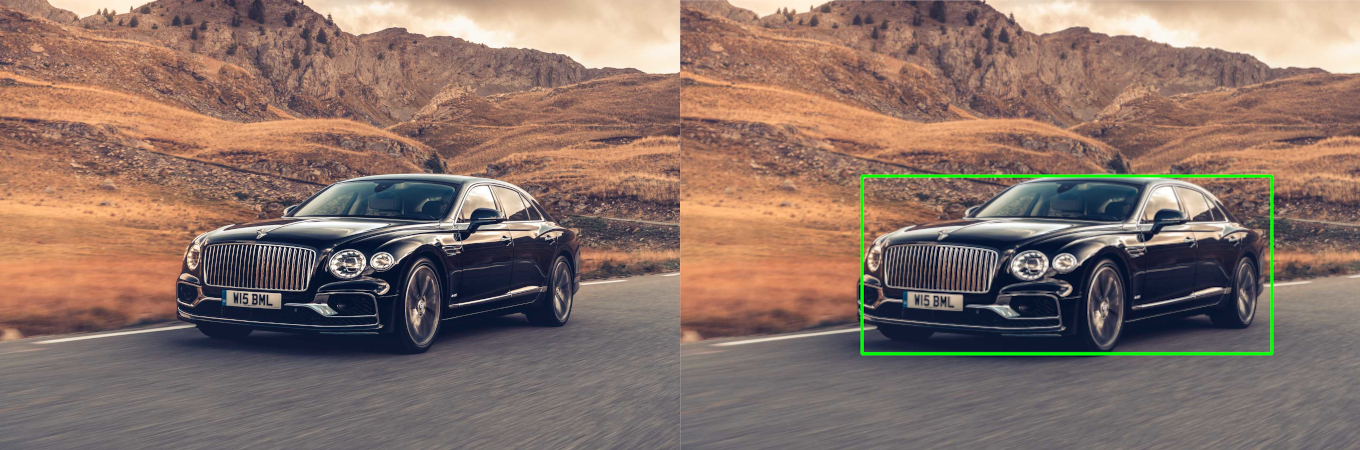
\includegraphics[scale=1.43]{img/detection_visualization.jpg}
    \end{center}
    \caption{Obraz przed i po detekcji samochodu\protect\footnotemark}
    \label{fig:cnn_arch_pic}
\end{figure}

\footnotetext{Użyte zdjęcie samochodu dostępne pod adresem:      \url{https://images.hgmsites.net/hug/2020-bentley-flying-spur_100720091_h.jpg}}

\subsection{Wycięcie obiektów oraz wyodrębnienie cech znaczących}
Po operacji detekcji, wycinamy wszystkie instancje odnalezionych samochodów z obrazu na podstawie otrzymanych w trakcie detekcji współrzędnych. W tym celu posługujemy się biblioteką numpy. Dokonane jest to, przez proste zapisanie do osobnej tablicy obrazu okrojonego (z ang. array slicing) o współrzędne otrzymane w trakcie detekcji.

\begin{lstlisting}[language=Python, caption=Wycięcie obiektów]
image_cropped = image[y: y + h, x: x + w]
\end{lstlisting}
\begin{math}
x
\end{math}
- odległość górnego, lewego wierzchołka prostokąta opisanego na wykrytym obiekcie od lewej granicy obrazu oryginalnego\\
\begin{math}
y
\end{math}
- odległość górnego, lewego wierzchołka prostokąta opisanego na wykrytym obiekcie od górnej granicy obrazu oryginalnego\\
\begin{math}
w
\end{math}
- szerokość prostokąta opisanego na wykrytym obiekcie\\
\begin{math}
h
\end{math}
- wysokość prostokąta opisanego na wykrytym obiekcie\\

Biblioteka OpenCV zawiera metodę \textbf{calcHist} służącą do ekstrakcji histogramu kolorów z danych liczbowych obrazu. Otrzymujemy w ten sposób informację o nasyceniu kanałów R, G oraz B w obrazie, bez ich lokalizacji w obrazie. To znacznie zmniejsza wielkość wynikowej tablicy liczbowej, a więc poprawia wydajność trenowania i działania perceptronu wielowarstwowego.

\begin{lstlisting}[language=Python, caption=Wyodrębnienie cech znaczących]
 features = []

hist = cv2.calcHist(
    [image_cropped], # Dane liczbowe obiektu wycietego z obrazu
    [0, 1, 2], # Ilosc kanalow (3 kanaly - RGB)
    None, # Maska
    (16, 16, 16),  # Rozdzielczosc dla kazdego z kanalow
    [0, 256, 0, 256, 0, 256]) # Zakres kolorow ktore chcemy wziac pod uwage dla kazdego z kanalow
hist = cv2.normalize(hist, hist).flatten() # Normalizacja histogramu

features.extend(hist)
\end{lstlisting}

Zmienna \textbf{features} (typu listy) przechowuje dane liczbowe histogramu kolorów otrzymanego w trakcie operacji wyodbrębniania cech znaczących.

\subsection{Stworzenie modelu uczenia maszynowego}

Biblioteka \textbf{scikit-learn} pozwala na implementację dowolnej konfiguracji uczenia maszynowego w prosty i przejrzysty sposób. Użyta konfiguracja modelu została uzyskana eksperymentalnie. Proces szukania owych parametrów został opisany w następnej sekcji (\ref{sec:grid}). Dzięki użyciu zaszytych w bibliotece scikit-learn metod oraz klas, można w następujący sposób zdefiniować model perceptronu wielowarstwowego:

\begin{lstlisting}[language=Python, caption=Definiowanie modelu MLP]
from sklearn.neural_network import MLPClassifier
mlp = MLPClassifier(
        hidden_layer_sizes=(100, 50, 25), # 1
        max_iter=5000, # 2
        solver="adam", # 3
        activation="relu", # 4
        learning_rate="adaptive", # 5)
\end{lstlisting}

\null{}

Zdefiniowany w ten sposób model MLP cechuje się:
\begin{enumerate}
    \item Trzema warstwami ukrytymi, o liczebnościach kolejno 100, 50 i 25 sztucznych neuronów
    \item Maksymalną ilością 5 tysięcy powtórzeń modyfikacji wag na podstawie funkcji kosztu (MSE).
    \item Funkcją optymalizacji wag w postaci algorytmu działającego na podstawie gradientu stochastycznego (z ang. stochastic gradient)
    \item Funkcją aktywacji Rectified Linear Unit (ReLU)
    \item Zmiennym współczynnikiem uczenia. Wagi są z każdą iteracją dopasowywane z zmienną czułością, pozwalając na ich dokładniejsze dostrojenie.
\end{enumerate}

\subsection{Dobór parametrów modelu MLP}
\label{sec:grid}

Użyte w definiowaniu modelu parametry nie są oczywiście przypadkowe. W celu znalezienia parametrów najbliższych optymalnym (w przystępnym czasie) możemy posłużyć się klasą \textbf{GridSearchCV} dostępną w module \textbf{scikit-learn}. 

W swojej istocie, klasa ta działa następująco: po podaniu jej przestrzeni parametrów, konstruuje z wielu wariacji zadanych parametrów nowe modele, trenuje je, a następnie generuje dla nich metryki jakościowe. 

Po okresie tworzenia, trenowania i walidacji jakości modeli, w zmiennej \textbf{best\_params\_} przechowywane są parametry modelu, który wykazał się najwyższymi wynikami.

\begin{lstlisting}[language=Python, caption=Przykład użycia klasy GridSearchCV]
from sklearn.model_selection import GridSearchCV
parameter_space = {
    'hidden_layer_sizes': [(100, 50, 25), (100, 70, 40, 10),
                (100, 45, 10), (70, 35, 17), (70, 52, 35, 17)],
    'max_iter': [5000],
    'activation': ['tanh', 'relu'],
    'solver': ['sgd', 'adam'],
    'alpha': [0.0001, 0.05, 1e-3],
    'learning_rate': ['constant','adaptive'],
}
best_mlp = GridSearchCV(MLPClassifier(), parameter_space,  
            n_jobs=-1, # Ilosc uzywanych procesorow logicznych (-1 oznacza uzycie wszystkich dostepnych w systemie)
            verbose=4) # logowanie duzej ilosci komunikatow
best_mlp.fit(X_train, y_train) # trenowanie i walidacja nowych modeli

print(mlp_from_grid.best_params_)
\end{lstlisting}

Parametry zawierane w przestrzeni są wybierane bez konkretnej reguły, a raczej na podstawie doświadczenia i intuicji. Trudno przewidzieć jak połączenia poszczególnych wartości mogą ze sobą współgrać w skomplikowanych przypadkach, dlatego potrzebujemy programowej metody, która uzasadnia wybrane przez nas parametry modelu.\\

Warto wspomnieć, iż konstruktor klasy GridSearchCV pozwala na konfigurację związaną z współbieżnością procesu trenowania modeli. Możemy podać ilość procesorów logicznych, które mają być przeznaczone na rzecz wykonania trenowań lub pozwolić tej klasie na programowe wykrycie ilości dostępnych procesorów logicznych w naszym systemie i utworzenie właśnie tylu procesów.
    
\pagebreak
    
\subsection{Trenowanie modelu i przewidywanie}
Korzystając z wcześniej zdefiniowanego obiektu modelu perceptronu wielowarstwowego możemy wytrenować model na podstawie przetworzonych danych (po detekcji, wycięciu oraz ekstrakcji histogramu kolorów). Do tego użyjemy metody \textbf{fit}, której podajemy jako argumenty wspomniane dane oraz ich etykiety.

Po wytrenowaniu modelu, możemy za jego pomocą zacząć generalizować kolory aut nowych instancjach obrazów samochodów. Wtedy jako argument metody \textbf{predict} podajemy przetworzone dane nowego obrazu. Metoda zwróci nam wówczas wykryty kolor samochodu.

\begin{lstlisting}[language=Python, caption=Trenowanie modelu i przewidywanie]
mlp.fit(X_train, y_train)

y_pred = mlp.predict(X_test)
\end{lstlisting}
\begin{math}
X\_train
\end{math}
- dane trenujące\\
\begin{math}
X\_test
\end{math}
- dane testowe\\
\begin{math}
y\_train
\end{math}
- etykiety danych trenujących\\
\begin{math}
y\_pred
\end{math}
- przewidziany wynik na podstawie danych testowych\\


% \begin{figure}[h!]
%     \begin{center}
%         
\includegraphics[scale=0.5]{img/technologie.png}        
%     \end{center}
%     \caption{Użyte technologie}
%     \label{fig:użyte technologie}
% \end{figure}
\section{Wyniki części praktycznej}
W poprzednim rozdziale, omówione zostały operacje, techniki oraz technologie zastosowane przy implementacji poszczególnych modułów algorytmu. Po połączeniu ich w całość, otrzymujemy algorytm pozwalający na wykrycie samochodu w obrazie oraz rozpoznanie jego koloru. Aby móc ocenić poprawność oraz szybkość jego działania możemy posłużyć się wachlarzem przeznaczonych do tego celu metryk. 

Pierwsza kategoria testów to testy \textbf{funkcjonalne} - mówią one o tym, w jakim stopniu algorytm spełnia powierzone mu zadanie. 

Następnie przybliżony zostanie aspekt \textbf{wydajnościowy} wynikowego programu - to jak szybko działa jako zintegrowana całość, ale również wydajność jego wyodrębnionych modułów. W ten sposób możemy wywnioskować, które operacje należałoby zoptymalizować, by przynieść największy zysk wydajnościowy.

\subsection{Testy funkcjonalne}
Zadaniem zaprojektowanego algorytmu jest rozpoznawanie koloru samochodów osobowych z obrazu. Aby móc porównać ze sobą jakość i działanie wielu różnych implementacji opartych o uczenie maszynowe w jednolity sposób, ustandaryzowano kilka podstawowych metryk jakościowych. 

\subsubsection{Standardowe metryki}
\begin{description}
\item \textbf{Macierz pomyłek} (z ang. confusion matrix) - to podstawa do wyznaczenia metryk jakościowych uczenia maszynowego. Jest to macierz, która dla dwóch klas (prawda lub fałsz) przedstawia wartości:
\begin{description}
\item \textbf{Prawdziwy Pozytyw} (\textbf{TP} z ang. True Positive) - to prawidłowo sklasyfikowany wynik pozytywny.
\item \textbf{Prawdziwy Negatyw} (\textbf{TN} z ang. True Negative) - to prawidłowo sklasyfikowany wynik negatywny.
\item \textbf{Fałszywy Pozytyw} (\textbf{FP} z ang. False Positive) - to nieprawidłowo sklasyfikowany wynik pozytywny.
\item \textbf{Fałszywy Negatyw} (\textbf{FN} z ang. False Negative) - to nieprawidłowo sklasyfikowany wynik negatywny.
\end{description}

Macierz pomyłek przybiera rozmiary NxN, gdzie N to liczba klas.

\begin{table}[]
\begin{center}
\begin{tabular}{lc|cc|}
\cline{3-4}
\multicolumn{2}{l|}{\multirow{2}{*}{}}                                                                       & \multicolumn{2}{c|}{Przewidziany wynik}                                                                                                          \\ \cline{3-4} 
\multicolumn{2}{l|}{}                                                                                        & \multicolumn{1}{c|}{Prawda}                                                       & Fałsz                                                        \\ \hline
\multicolumn{1}{|c|}{\multirow{2}{*}{\begin{tabular}[c]{@{}c@{}}Prawdziwy\\ \\ wynik\end{tabular}}} & Prawda & \multicolumn{1}{c|}{\begin{tabular}[c]{@{}c@{}}Prawdziwy\\ Pozytyw\end{tabular}} & \begin{tabular}[c]{@{}c@{}}Fałszywy\\ Pozytyw\end{tabular}   \\ \cline{2-4} 
\multicolumn{1}{|c|}{}                                                                              & Fałsz & \multicolumn{1}{c|}{\begin{tabular}[c]{@{}c@{}}Fałszywy\\ Negatyw\end{tabular}}   & \begin{tabular}[c]{@{}c@{}}Prawdziwy \\ Negatyw\end{tabular} \\ \hline
\end{tabular}
\caption{Macierz pomyłek o rozmiarze 2x2}
\label{tab:Confusion2x2}
\end{center}
\end{table}

\pagebreak

\item \textbf{Dokładność} (z ang. accuracy) - to najpowszechniejsza miara jakości klasyfikacji. Jest to stosunek obiektów sklasyfikowanych poprawnie do wszystkich elementów zbioru. 
\begin{center}
\resizebox{0.45\hsize}{!}{
dokładność $= \frac{TP + TN}{TP + FP + FN + TN}$
}
\end{center}

\item \textbf{Precyzja} (z ang. precision) - to stosunek prawidłowo przewidzianych elementów klasy do wszystkich elementów zbioru sklasyfikowanych jako element tej klasy.
\begin{center}
\resizebox{0.3\hsize}{!}{
precyzja $= \frac{TP}{TP + FP}$
}
\end{center}

\item \textbf{Czułość} (z ang. recall) - to stosunek prawidłowo przewidzianych elementów klasy do wszystkich faktycznie należących do niej elementów.
\begin{center}
\resizebox{0.3\hsize}{!}{
czułość $= \frac{TP}{TP + FN}$
}
\end{center}

\item \textbf{Miara F$_{1}$} (z ang. F1 score) - to średnia harmoniczna precyzji i czułości.
\begin{center}
\resizebox{0.4\hsize}{!}{
F$_{1}$ $= \frac{2 \cdot precyzja \cdot czulosc}{precyzja + czulosc}$
}
\end{center}

\item \textbf{Wsparcie} (z ang. support) - to liczba elementów klasy w zbiorze, na podstawie których wyliczone zostały metryki dla danej klasy.
\end{description}

\subsubsection{Wyniki i wnioski}
Dla przypomnienia, w skład użytego zbioru danych wchodzi 8 klas kolorów. Macierz pomyłek, która opisuje klasyfikacje zaimplementowanego modelu ma zatem rozmiar 8x8.

\begin{figure}[h!]
    \begin{center}
        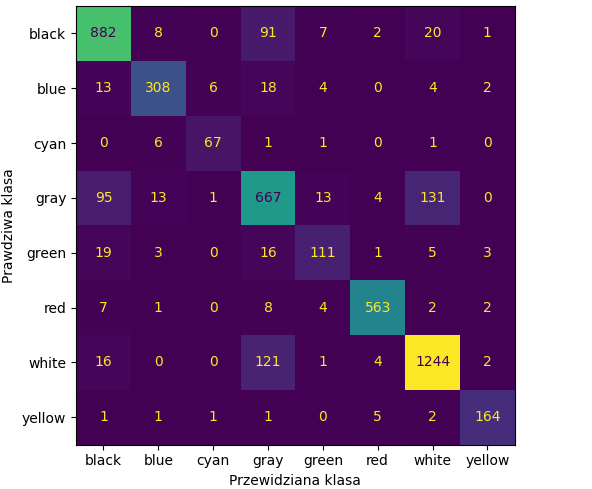
\includegraphics[scale=0.87]{img/confusion_matrix.png}        
    \end{center}
    \caption{Wynikowa macierz pomyłek}
    \label{fig:confusion_matrix}
\end{figure}

Wartości liczbowe zawarte w takiej macierzy pomyłek (Rysunek \ref{fig:confusion_matrix}) są jednak mało obrazowe. Jest tak, ponieważ każda z klas ma inne wsparcie. (Tabela \ref{tab:support})

\begin{table}[h!]
\begin{center}
\begin{tabular}{|l|l|l|l|l|l|l|l|}
\hline
Biały                      & Czarny                    & Szary                    & Czerwony                 & Niebieski                & Żółty                    & Zielony                  & Cyjanowy                \\ \hline
\multicolumn{1}{|c|}{1388} & \multicolumn{1}{c|}{1011} & \multicolumn{1}{c|}{924} & \multicolumn{1}{c|}{587} & \multicolumn{1}{c|}{355} & \multicolumn{1}{c|}{175} & \multicolumn{1}{c|}{158} & \multicolumn{1}{c|}{76} \\ \hline
\end{tabular}
\caption{Wsparcie klas}
\label{tab:support}
\end{center}
\end{table}

\begin{table}[h!]
\begin{center}
\begin{tabular}{|c|c|c|c|c|c|c|c|}
\hline
Biały & Czarny & Szary & Czerwony & Niebieski & Żółty & Zielony & Cyjanowy \\ \hline
4742  & 3418   & 3046  & 1941     & 1086      & 581   & 482     & 281      \\ \hline
\end{tabular}
\caption{Ilość elementów w każdej z klas}
\label{tab:classes_count}
\end{center}
\end{table}

Całkowite wsparcie, czyli ilość danych zbioru testowego, to \textbf{30\%} całkowitej ilości obrazów w zbiorze. Ta proporcja nie jest do końca zachowana dla każdej z klas i waha się w granicach \textbf{27,05\%} i \textbf{32,78\%}.

Możemy zatem w celu osiągnięcia bardziej obrazowej wizualizacji znormalizować macierz, tak, aby wyświetlane w niej wartości były niezależne od wsparcia poszczególnych klas.

\begin{figure}[h!]
    \begin{center}
        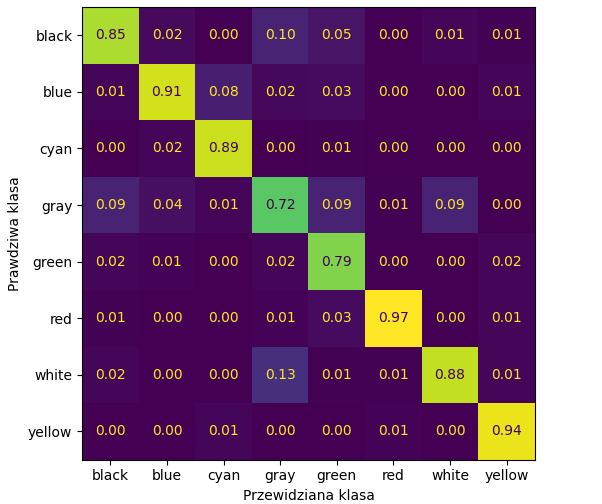
\includegraphics[scale=0.87]{img/confusion_matrix_new.png}        
    \end{center}
    \caption{Znormalizowana macierz pomyłek wobec ilości elementów przewidzianych jako należące do danej klasy}
    \label{fig:confusion_matrix_norm}
\end{figure}

\pagebreak

Z tak sformatowanej macierzy pomyłek (Rysunek \ref{fig:confusion_matrix_norm}) widzimy, że relatywnie najgorzej klasyfikowane były elementy klas kolorów: \textbf{zielony} oraz \textbf{szary}, a najwyższą jakościowo klasyfikacją wykazuje się klasa koloru \textbf{czerwonego}. Kolor szary najczęściej był mylony z kolorem (malejąco) białym, czarnym oraz zielonym. Natomiast kolor zielony najczęściej był mylony z kolorem zielonym oraz czarnym.
Podobny trend jest zauważalny na podstawie pozostałych metryk zawartych w poniższej tabeli (Tabela \ref{tab:metrics}).


\begin{table}[h!]
\begin{center}
\begin{tabular}{ccccc}
\cline{2-5}
\multicolumn{1}{c|}{}           & \multicolumn{1}{c|}{Precyzja} & \multicolumn{1}{c|}{Czułość} & \multicolumn{1}{c|}{Miara F1} & \multicolumn{1}{c|}{Wsparcie} \\ \hline
\multicolumn{1}{|c|}{Biały}     & \multicolumn{1}{c|}{0.88}     & \multicolumn{1}{c|}{0.90}    & \multicolumn{1}{c|}{0.89}     & \multicolumn{1}{c|}{1388}     \\ \hline
\multicolumn{1}{|c|}{Czarny}    & \multicolumn{1}{c|}{0.85}     & \multicolumn{1}{c|}{0.87}    & \multicolumn{1}{c|}{0.86}     & \multicolumn{1}{c|}{1011}     \\ \hline
\multicolumn{1}{|c|}{Szary}     & \multicolumn{1}{c|}{0.72}     & \multicolumn{1}{c|}{0.72}    & \multicolumn{1}{c|}{0.72}     & \multicolumn{1}{c|}{924}      \\ \hline
\multicolumn{1}{|c|}{Czerwony}  & \multicolumn{1}{c|}{0.97}     & \multicolumn{1}{c|}{0.96}    & \multicolumn{1}{c|}{0.97}     & \multicolumn{1}{c|}{587}      \\ \hline
\multicolumn{1}{|c|}{Niebieski} & \multicolumn{1}{c|}{0.91}     & \multicolumn{1}{c|}{0.87}    & \multicolumn{1}{c|}{0.89}     & \multicolumn{1}{c|}{355}      \\ \hline
\multicolumn{1}{|c|}{Żółty}     & \multicolumn{1}{c|}{0.94}     & \multicolumn{1}{c|}{0.94}    & \multicolumn{1}{c|}{0.94}     & \multicolumn{1}{c|}{175}      \\ \hline
\multicolumn{1}{|c|}{Zielony}   & \multicolumn{1}{c|}{0.79}     & \multicolumn{1}{c|}{0.70}    & \multicolumn{1}{c|}{0.74}     & \multicolumn{1}{c|}{158}      \\ \hline
\multicolumn{1}{|c|}{Cyjanowy}  & \multicolumn{1}{c|}{0.89}     & \multicolumn{1}{c|}{0.88}    & \multicolumn{1}{c|}{0.89}     & \multicolumn{1}{c|}{76}       \\ \hline
\multicolumn{1}{|c|}{Średnia}   & \multicolumn{1}{c|}{0.87}     & \multicolumn{1}{c|}{0.85}    & \multicolumn{1}{c|}{0.86}     & \multicolumn{1}{c|}{4674}     \\ \hline
\multicolumn{1}{l}{}            & \multicolumn{1}{l}{}          & \multicolumn{1}{l}{}         & \multicolumn{1}{l}{}          & \multicolumn{1}{l}{}          \\ \hline
\multicolumn{2}{|l|}{\textbf{Dokładność}}                       & \multicolumn{3}{c|}{\textbf{86.24\%}}                                                        \\ \hline
\end{tabular}
\caption{Metryki jednowymiarowe}
\label{tab:metrics}
\end{center}
\end{table}

\pagebreak

Niskie rezultaty jakościowe dla najgorzej klasyfikowanych kolorów, są spowodowane w dużej mierze degeneracją i błędami w zbiorze danych. Jako dowód można przytoczyć zrzut ekranu zawartości folderu, w którym znajdują się zdjęcia samochodów z etykietą koloru \textbf{"\null{}green"} (zielone auta):

\begin{figure}[h!]
    \begin{center}
        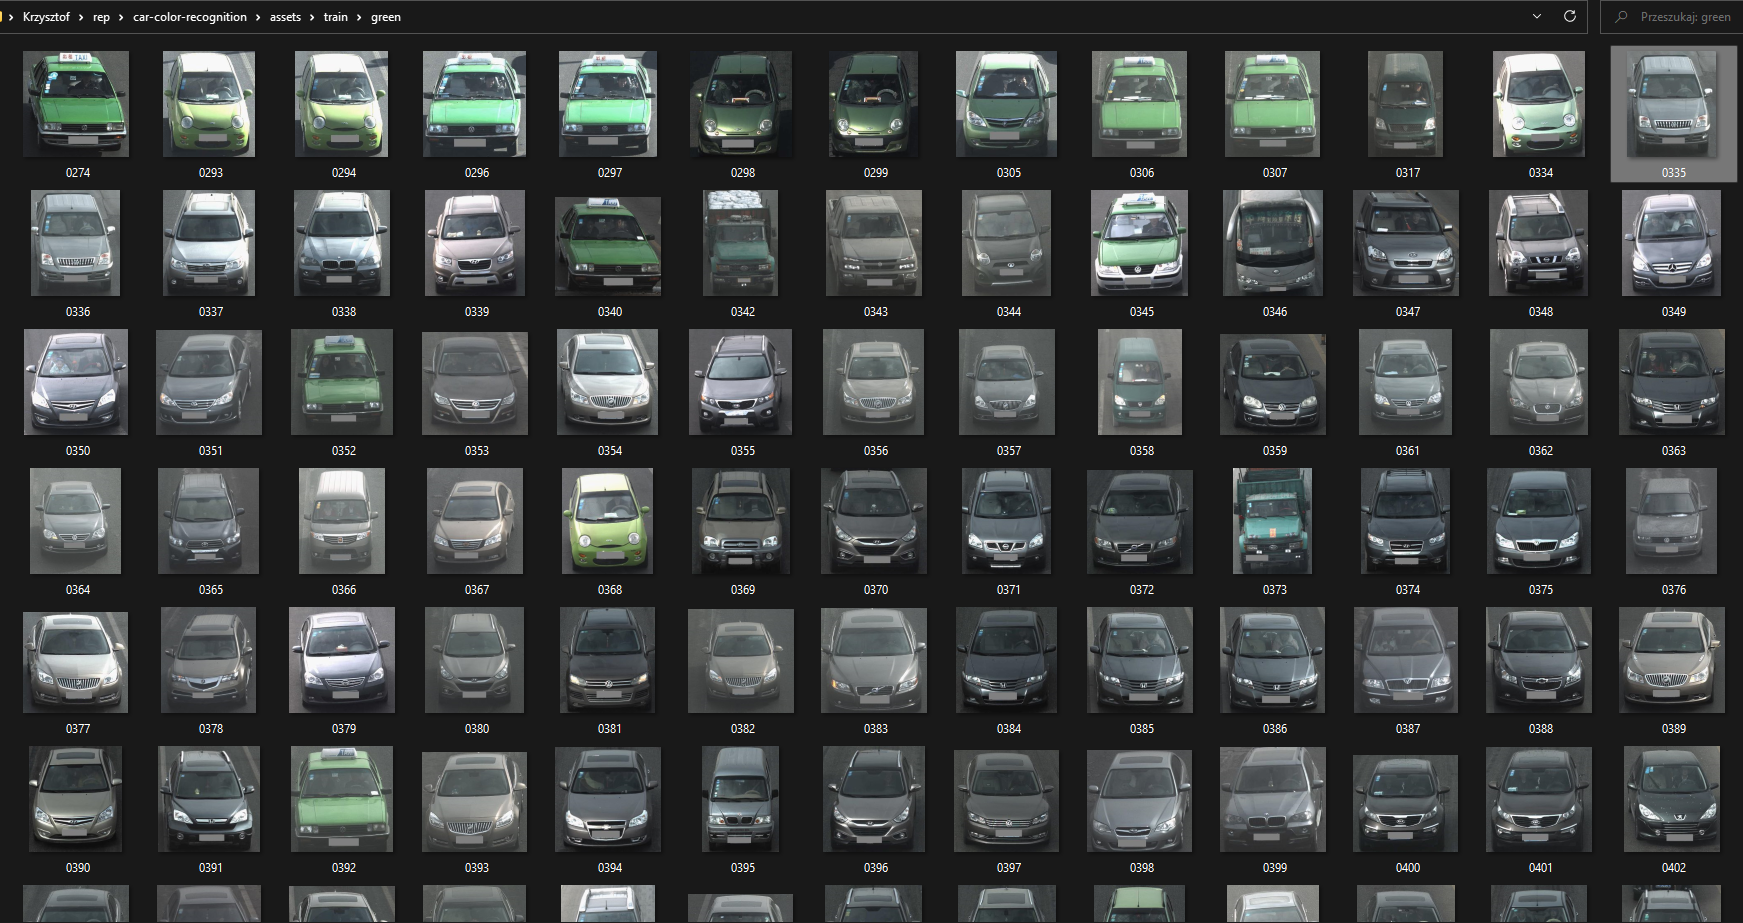
\includegraphics[scale=0.31]{img/green_cars_xd.png}        
    \end{center}
    \caption{Katalog zawierający zdjęcia aut opisane jako zielone}
    \label{fig:green_cars_xd}
\end{figure}

Ogromna ilość z widocznych w katalogu zdjęć, zawiera auta o kolorze szarym i czarnym, a \textbf{nie zielonym}. Nie powinno być więc zaskoczeniem, iż auta zielone są mylone często z autami czarnymi oraz szarymi, skoro duża część etykiet jest kompletnie \underline{źle przypisana}. 

\begin{figure}[h!]
    \begin{center}
        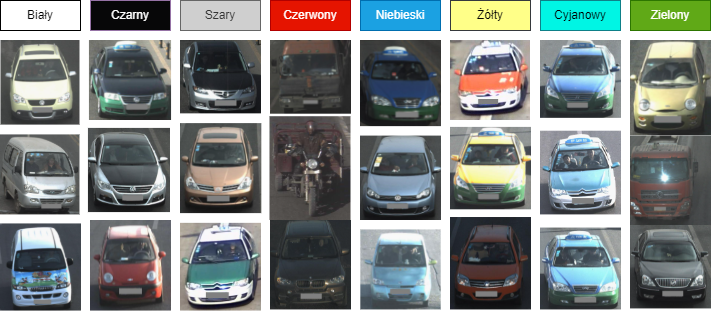
\includegraphics[scale=0.57]{img/cars_bad_colors.png}        
    \end{center}
    \caption{Po 3 przykładowe, źle przypisane elementy dla każdej z klas}
    \label{fig:bad_cars_xd}
\end{figure}

Podobnie jak kolor zielony, inne klasy mają dużo źle przypisanych elementów, co widać na powyższym rysunku (Rysunek \ref{fig:bad_cars_xd}). Do wizualizacji zostało wybrane tylko kilka najbardziej rażących przypadków z każdej z klas (bez powtórek tego samego auta - mimo, że każde występuje kilku lub kilkunastokrotnie w zbiorze oryginalnym).

Aby zniwelować ten problem, zbiór danych został manualnie wyczyszczony, to znaczy pozbawiony zdjęć, których etykiety były sprzeczne z rzeczywistością obrazu. Takich przypadków było niestety dużo, co poskutkowało znacznym zmniejszeniem się wynikowej ilości elementów zbioru. Zmniejszyła się ona z ponad \textbf{15 tys.} obrazów, do tylko \textbf{6415} zdjęć.

\begin{table}[h!]
\begin{center}
\begin{tabular}{|c|c|c|c|c|c|c|c|}
\hline
Biały & Czarny & Szary & Czerwony & Niebieski & Żółty & Cyjanowy & Zielony \\ \hline
739   & 726    & 469   & 145      & 66        & 38    & 32       & 31      \\ \hline
\end{tabular}
\caption{Wsparcie klas po czyszczeniu zbioru danych}
\label{tab:support_reword}
\end{center}
\end{table}

Stosunek podziału zbioru na dane trenujące i testowe został zmieniony z \textbf{70:30} do \textbf{65:35}, a mimo tego, wsparcie niektórych klas i tak stało się na tyle małe, że może ono budzić niepewność i podejrzliwość co do uzyskanych wyników jakościowych.

\begin{table}[h!]
\begin{center}
\begin{tabular}{|c|c|c|c|c|c|c|c|}
\hline
Biały & Czarny & Szary & Czerwony & Niebieski & Żółty & Cyjanowy & Zielony \\ \hline
2153  & 1972   & 1318  & 449      & 217       & 121   & 107      & 78      \\ \hline
\end{tabular}
\caption{Ilości elementów poszczególnych klas zbioru po jego czyszczeniu}
\label{tab:dataset_count_reword}
\end{center}
\end{table}

Po usunięciu ze zbioru obrazów o sprzecznych etykietach lub nie-akceptowalnych jakościowo zdjęć (takich, w których koloru auta nie rozpoznałby nawet człowiek), otrzymujemy następujące macierze pomyłek oraz metryki jednowymiarowe:

\begin{table}[h!]
\begin{center}
\begin{tabular}{crrrr}
\cline{2-5}
\multicolumn{1}{c|}{}           & \multicolumn{1}{c|}{Precyzja} & \multicolumn{1}{c|}{Czułość} & \multicolumn{1}{c|}{Miara F1} & \multicolumn{1}{c|}{Wsparcie} \\ \hline
\multicolumn{1}{|c|}{Biały}     & \multicolumn{1}{r|}{0.97}     & \multicolumn{1}{r|}{0.82}    & \multicolumn{1}{r|}{0.89}     & \multicolumn{1}{r|}{726}      \\ \hline
\multicolumn{1}{|c|}{Czarny}    & \multicolumn{1}{r|}{0.96}     & \multicolumn{1}{r|}{0.96}    & \multicolumn{1}{r|}{0.96}     & \multicolumn{1}{r|}{66}       \\ \hline
\multicolumn{1}{|c|}{Szary}     & \multicolumn{1}{r|}{0.91}     & \multicolumn{1}{r|}{0.93}    & \multicolumn{1}{r|}{0.92}     & \multicolumn{1}{r|}{32}       \\ \hline
\multicolumn{1}{|c|}{Czerwony}  & \multicolumn{1}{r|}{0.99}     & \multicolumn{1}{r|}{0.99}    & \multicolumn{1}{r|}{0.99}     & \multicolumn{1}{r|}{469}      \\ \hline
\multicolumn{1}{|c|}{Niebieski} & \multicolumn{1}{r|}{0.89}     & \multicolumn{1}{r|}{0.94}    & \multicolumn{1}{r|}{0.91}     & \multicolumn{1}{r|}{31}       \\ \hline
\multicolumn{1}{|c|}{Żółty}     & \multicolumn{1}{r|}{0.97}     & \multicolumn{1}{r|}{0.82}    & \multicolumn{1}{r|}{0.89}     & \multicolumn{1}{r|}{145}      \\ \hline
\multicolumn{1}{|c|}{Zielony}   & \multicolumn{1}{r|}{0.93}     & \multicolumn{1}{r|}{0.81}    & \multicolumn{1}{r|}{0.86}     & \multicolumn{1}{r|}{739}      \\ \hline
\multicolumn{1}{|c|}{Cyjanowy}  & \multicolumn{1}{r|}{0.91}     & \multicolumn{1}{r|}{0.94}    & \multicolumn{1}{r|}{0.92}     & \multicolumn{1}{r|}{38}       \\ \hline
\multicolumn{1}{|c|}{Średnia}   & \multicolumn{1}{r|}{0.94}     & \multicolumn{1}{r|}{0.92}    & \multicolumn{1}{r|}{0.93}     & \multicolumn{1}{r|}{2246}     \\ \hline
\multicolumn{1}{l}{}            & \multicolumn{1}{l}{}          & \multicolumn{1}{l}{}         & \multicolumn{1}{l}{}          & \multicolumn{1}{l}{}          \\ \hline
\multicolumn{2}{|l|}{\textbf{Dokładność}}                       & \multicolumn{3}{c|}{\textbf{95.32\%}}                                                        \\ \hline
\end{tabular}
\caption{Metryki jednowymiarowe po czyszczeniu zbioru danych}
\label{tab:metrics_reword}
\end{center}
\end{table}

\pagebreak

\begin{figure}[h!]
    \begin{center}
        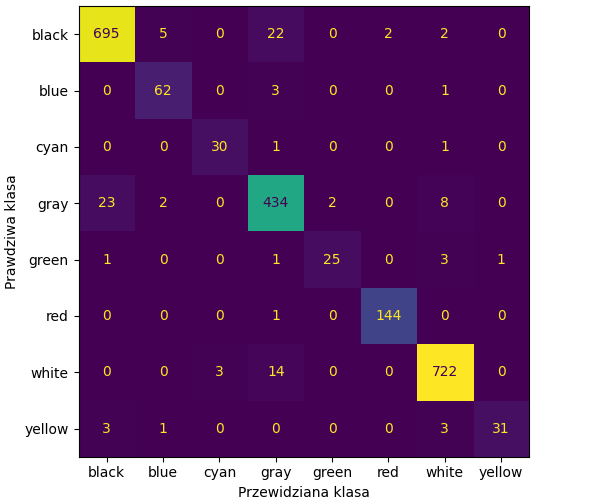
\includegraphics[scale=0.78]{img/confusion_matrix_rework.png}        
    \end{center}
    \caption{Macierz pomyłek po czyszczeniu zbioru}
    \label{fig:confusion_rework}
\end{figure}

\begin{figure}[h!]
    \begin{center}
        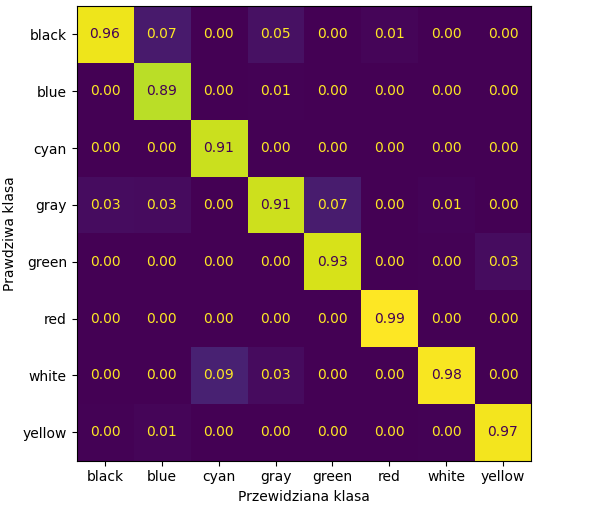
\includegraphics[scale=0.78]{img/confusion_matrix_new_rework.png}
    \end{center}
    \caption{Znormalizowana macierz pomyłek po czyszczeniu zbioru}
    \label{fig:confusion_new_rework}
\end{figure}

\pagebreak

Są to bardzo obiecujące wyniki, przewyższające te, osiągnięte w realizacji opisanych wcześniej prac naukowych, które korzystają z tego zbioru danych. Zbiór danych przy trenowaniu modelu jest dzielony na dwa osobne, niezależne podzbiory - \textbf{trenujący} i \textbf{testujący}. Przez ten fakt możemy z wysokich wyników jakościowych wysnuć wniosek, że model poprawnie uogólnia nowo napotkane, nieznane mu przypadki aut.

Trzeba jednak mieć na uwadze, że wszystkie podane metryki są miarą tego jak dobrze model generalizuje auta ze zdjęć zbioru testowego. Zatem dobrze wypadający na takich testach model cechujący się dokładnością nieco ponad \textbf{95\%}, może wykazywać się ubogą jakością generalizacji na danych spoza zbioru testowego, na przykład danych rzeczywistych.

\subsection{Testy wydajnościowe}
Oprócz informacji o tym \textbf{co?}, \textbf{jak?} i \textbf{w jakim stopniu?} robi algorytm, chcielibyśmy uzyskać również wgląd w to w jakim czasie potrafi osiągnąć daną funkcjonalność. Kroki algorytmu wpływają w jego holistyczny czas wykonania w różnym stopniu. Przetestowane pod kątem wydajnościowym zostaną zatem najbardziej znaczące moduły, takie jak trenowanie modelu, detekcja pojazdów oraz działanie programu jako całość.

Wszystkie parametry czasowe były pozyskiwane na komputerze stacjonarnym z użyciem jedynie \textbf{CPU}. Jest to spowodowane poważnymi problemami z uruchomieniem modułu OpenCV w wersji używającej wspomagania dedykowanego układu GPU z rdzeniami CUDA w celu dalszego zrównoleglenia obliczeń. 

\subsubsection{Czas trenowania modelu}
Istnieją dwie wersje modelu perceptronu wielowarstwowego, którego używa algorytm. Jest to model przed i po czyszczeniu zbioru danych. Przed czyszczeniem zbioru, składał się on z \textbf{15579} obrazów. Wtedy czas uczenia modelu wahał się w granicach \textbf{260-310 sekund}, czyli około czterech minut.

Po czyszczeniu zbioru danych, jego liczebność zmalała do 6415 obrazów. Przy takiej ilości zdjęć, czas potrzebny na wytrenowanie perceptronu wielowarstwowego zawierał się w granicach \textbf{70-120 sekund}.

Oba czasy, przed i po zmianie zbioru danych, są o kilka rzędów niższe od czasu potrzebnego na trenowanie modelu w rozwiązaniach opartych o CNN, które przy około 8 tysiącach obrazów trwało niemal 4 dni (na potężnym komputerze dysponującym drogimi zestawami GPU!), a tak czy inaczej uzyskało wynik \textbf{94\%} dokładności generalizacji, czyli \textbf{niższy o 1\%} od uzyskanego modelu.

\subsubsection{Szybkość detekcji}
Program pozwala nam na dokonanie detekcji samochodów osobowych na trzech typach danych wejściowych: z zapisanego na dysku obrazu, z zapisanego na dysku obrazu wideo lub obrazu na żywo z systemowego wejścia wideo.

Dla obrazów stałych, miarą szybkości detekcji może być po prostu sumaryczny czas potrzebny na odnalezienie, obróbkę (wskazanie) oraz wyświetlenie obrazu wynikowego. Czas ten zawiera się w granicach \textbf{360-450 milisekund}, przy 20 próbach. Średnia czasu z wszystkich prób to: \textbf{387.2 milisekundy}.

Dla obrazów wideo oraz obrazu na żywo, obraną miarą szybkości detekcji są klatki na sekundę (FPS, z and. Frames per Second). Jednak miara FPS rzadko jest stała przez czas całość trwania wideo. Dlatego podana zostanie \textbf{wartość średnia} FPS, \textbf{mediana}, \textbf{wartość maksymalna} oraz \textbf{25.} oraz \textbf{75. centyl}.

\begin{description}
\item \textbf{Wideo nr1} - przypadek testowy numer 1. To 10 sekundowy film przedstawiający obraz z ruchomej kamery ulicznej pozycjonowanej nad czteropasmową drogą szybkiego ruchu z widokiem frontalnym na nadjeżdżające samochody osobowe. Na filmie przez pole widzenia kamery przejeżdża wiele aut i widocznych jest wiele innych obiektów przyulicznych. Rozdzielczość obrazu to 1280x720 pikseli, a oryginalna ilość klatek na sekundę to 29.97 FPS.

\item \textbf{Wideo nr2} - przypadek testowy numer 2. To krótkie, 5 sekundowe wideo, w którym widać od przodu wchodzące w zakręt i z niego wychodzące pojedyncze niebieskie auto. Dookoła widać dużo przedmiotów przyulicznych i roślinności. Rozdzielczość filmu to 960x540, w oryginale 30 FPS. 

\end{description}

\begin{table}[h!]
\begin{center}
\begin{tabular}{|l|l|l|}
\hline
\multicolumn{1}{|c|}{Miary FPS} & Wideo nr1 & Wideo nr2 \\ \hline
Średnia                         & \textbf{5.245}     & \textbf{5.040}     \\ \hline
Max                             & 5.579     & 5.465     \\ \hline
75.                             & 5.404     & 5.212     \\ \hline
Mediana                         & 5.265     & 5.151     \\ \hline
25.                             & 5.163     & 4.927     \\ \hline
\end{tabular}
\caption{Miary FPS detekcji z obrazu wideo dla dwóch przypadków testowych}
\label{tab:fps_detection}
\end{center}
\end{table}

\begin{figure}[h!]
    \begin{center}
        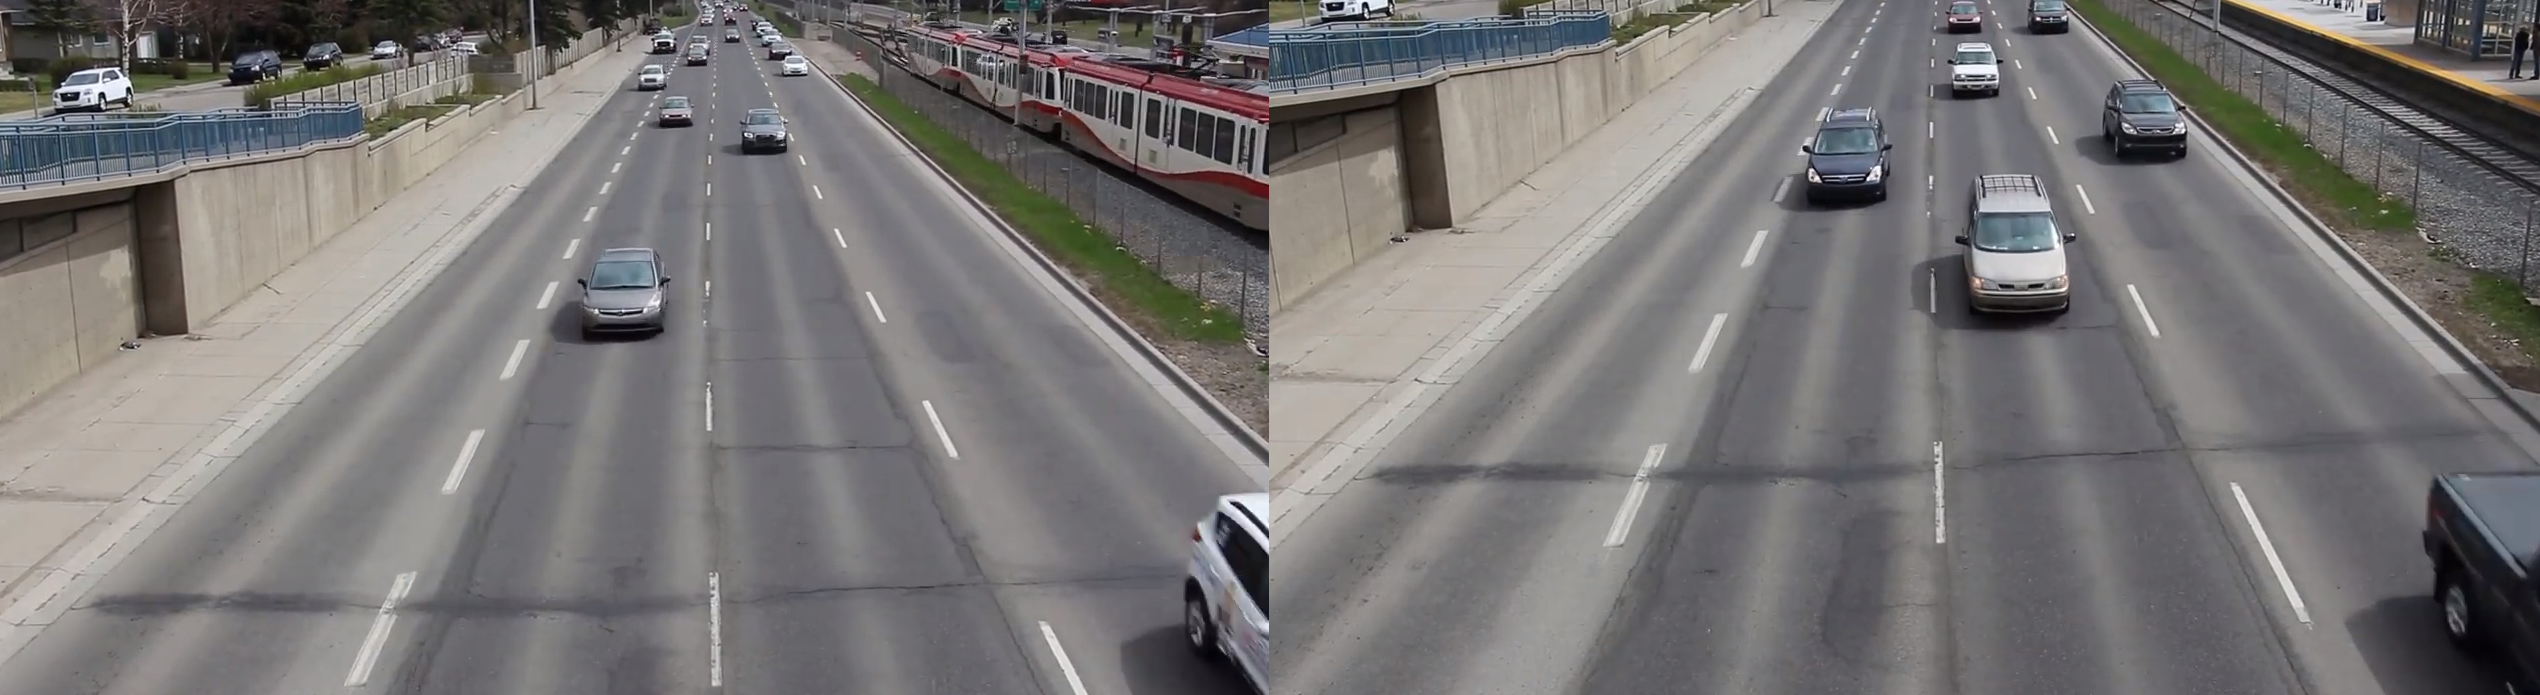
\includegraphics[scale=0.21]{img/cam1.png}
    \end{center}
    \caption{Dwa przykładowe ujęcia z przypadku testowego nr1}
    \label{fig:cam1}
\end{figure}

\begin{figure}[h!]
    \begin{center}
        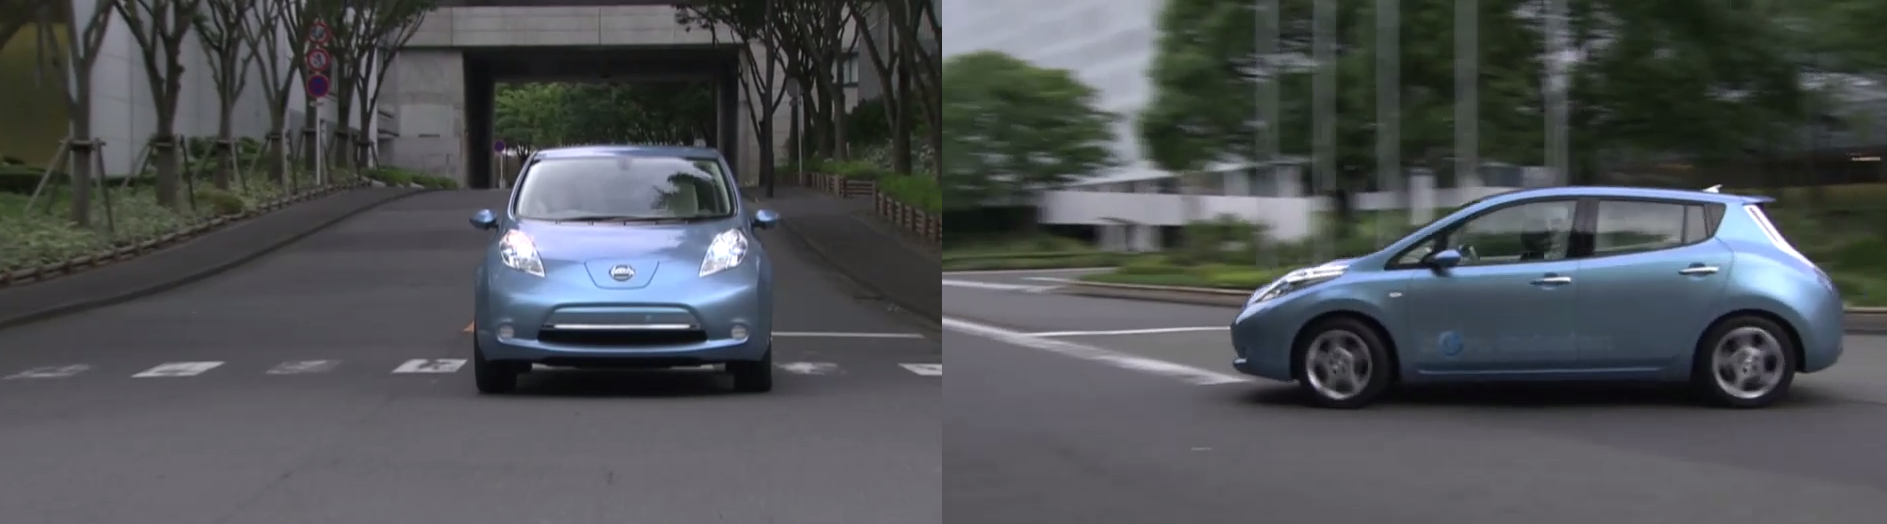
\includegraphics[scale=0.28]{img/cam2.png}
    \end{center}
    \caption{Dwa przykładowe ujęcia z przypadku testowego nr2}
    \label{fig:cam2}
\end{figure}

% Opis wynikow

\pagebreak

\subsubsection{Parametry czasowe rozpoznawania koloru samochodów}

Parametry czasowe działania całości algorytmu, czyli detekcji i rozpoznawania koloru samochodów osobowych już wytrenowanym modelem, pozyskiwane są analogiczne do parametrów czasowych samej detekcji.

Dla obrazów stałych, jest to czas potrzebny na użycie algorytmu na zdjęciach. Wartość tego czasu zawiera się w granicach \textbf{455-584 milisekund}, przy 20 próbach. Średnia czasu z wszystkich prób to: \textbf{483.1 milisekundy}.\\

Natomiast dla obrazów wideo jak i obrazu "\null{}na żywo", pozyskane parametry czasowe prezentują się następująco:

\begin{table}[h!]
\begin{center}
\begin{tabular}{|l|l|l|}
\hline
\multicolumn{1}{|c|}{Miary FPS} & Wideo nr1 & Wideo nr2 \\ \hline
Średnia                         & \textbf{4.571}     & \textbf{4.826}     \\ \hline
Max                             & 5.256     & 5.190     \\ \hline
75.                             & 4.877     & 4.993     \\ \hline
Mediana                         & 4.756     & 4.849     \\ \hline
25.                             & 4.540     & 4.774     \\ \hline
\end{tabular}%
\caption{Miary FPS działania pełnego algorytmu na obrazie wideo dla dwóch przypadków testowych}
\label{tab:fps_recog}
\end{center}
\end{table}

Widać zatem, iż to detekcja jest najbardziej obarczającą algorytm czasowo operacją. Zmniejszenie czasu potrzebnego na detekcję pod kątem oprogramowania, wiązałoby się z użyciem innych parametrów modelu detekcji, stworzeniem zupełnie innego modelu lub skorzystanie z zupełnie innego rozwiązania niż uczenie maszynowe. Inny sposób to podejście sprzętowe. Użycie układu GPU obsługującego technologie CUDA, w celu zrównoleglenia obliczeń znacznie wpłynęłoby na całościową szybkość działania algorytmu. 

Niestety, dostępne stacje robocze oraz zasoby komputerowe nie pozwalają mi na użycie układu GPU z moim programem. To znacznie zmniejsza atrakcyjność algorytmu w kontekście jego działania na obrazie wideo.
\section*{Podsumowanie} \addcontentsline{toc}{section}{Podsumowanie}

W pracy, udokumentowany został projekt i implementacja algorytmu umożliwiającego rozpoznawanie koloru samochodów osobowych. Przytoczone zostały podstawy teoretyczne, pozwalające zrozumieć i czerpać ze struktury oraz wyników otrzymanego programu. Przybliżenie użytych technologii i bibliotek zarysowało obraz tego w jaki sposób zostały programowo wcielone w życie operacje potrzebne do osiągnięcia zadanej funkcjonalności. 

Pozyskane wyniki zaprezentowały zalety modelu uczenia maszynowego w generalizowaniu koloru aut na podstawie dostępnego zbioru danych. Wysoka skuteczność modelu perceptronu wielowarstwowego, uzyskana została dzięki ręcznej filtracji zbioru danych, niwelując występujący w nim szum w postaci błędów ludzkich oraz nie-idealności jakościowej poszczególnych obrazów.

Program jest funkcjonalny i uniwersalny - działa na wielu rodzajach oraz formatach danych wejściowych i potrafi małym kosztem przedstawić multum metryk pozwalających na jego ewaluację oraz porównanie. Dalszą częścią rozwoju projektu, byłoby dalsze przystosowanie oraz uruchomienie go na systemie dysponującym układem GPU, co pozwoliłoby na znaczne przyspieszenie jego działania, zwłaszcza na danych wideo.

Oprócz tego, możliwe jest dokładniejsze dopasowanie konfiguracji modelu detekcji pod kątem wydajnościowym lub użycie innego rodzaju detekcji niż uczenie maszynowe.

\addcontentsline{toc}{section}{Literatura}
\bibliography{bibliography.bib}
\bibliographystyle{ieeetr}
\end{document}
